%===============================================================================
% LaTeX sjabloon voor de bachelorproef toegepaste informatica aan HOGENT
% Meer info op https://github.com/HoGentTIN/latex-hogent-report
%===============================================================================

\documentclass[dutch,dit,thesis]{hogentreport}

\usepackage{lipsum}  % For blind text, can be removed after adding actual content
\usepackage{subcaption}
\usepackage{listings}

\usepackage{xcolor}

\definecolor{codegreen}{rgb}{0,0.6,0}
\definecolor{codegray}{rgb}{0.5,0.5,0.5}
\definecolor{codepurple}{rgb}{0.58,0,0.82}
\definecolor{backcolour}{rgb}{0.95,0.95,0.92}

\lstdefinestyle{mystyle}{
    backgroundcolor=\color{backcolour},   
    commentstyle=\color{codegreen},
    keywordstyle=\color{magenta},
    numberstyle=\tiny\color{codegray},
    stringstyle=\color{codepurple},
    basicstyle=\ttfamily\footnotesize,
    breakatwhitespace=false,         
    breaklines=true,                 
    captionpos=b,                    
    keepspaces=true,                 
    numbers=left,                    
    numbersep=5pt,                  
    showspaces=false,                
    showstringspaces=false,
    showtabs=false,                  
    tabsize=2
}

\lstset{style=mystyle}

%% Pictures to include in the text can be put in the graphics/ folder
\graphicspath{{../graphics/}}

%% For source code highlighting, requires pygments to be installed
%% Compile with the -shell-escape flag!
%% \usepackage[chapter]{minted}
%% If you compile with the make_thesis.{bat,sh} script, use the following
%% import instead:
\usepackage[chapter]{minted}
\usemintedstyle{solarized-light}

%% Formatting for minted environments.
\setminted{%
    autogobble,
    frame=lines,
    breaklines,
    linenos,
    tabsize=4
}

%% Ensure the list of listings is in the table of contents
\renewcommand\listoflistingscaption{%
    \IfLanguageName{dutch}{Lijst van codefragmenten}{List of listings}
}
\renewcommand\listingscaption{%
    \IfLanguageName{dutch}{Codefragment}{Listing}
}
\renewcommand*\listoflistings{%
    \cleardoublepage\phantomsection\addcontentsline{toc}{chapter}{\listoflistingscaption}%
    \listof{listing}{\listoflistingscaption}%
}

% Other packages not already included can be imported here

%%---------- Document metadata -------------------------------------------------
\author{Ian Daelman}
\supervisor{Dhr. T. Aelbrecht}
\cosupervisor{Dhr. K. Mekers}
\title{Hulp voor de Helpdesk: Virtuele Assistenten als Ondersteuningstool.}
\academicyear{\advance\year by -1 \the\year--\advance\year by 1 \the\year}
\examperiod{1}
\degreesought{\IfLanguageName{dutch}{Professionele bachelor in de toegepaste informatica}{Bachelor of applied computer science}}
\partialthesis{false} %% To display 'in partial fulfilment'
%\institution{Internshipcompany BVBA.}

%% Add global exceptions to the hyphenation here
\hyphenation{back-slash}

%% The bibliography (style and settings are  found in hogentthesis.cls)
\addbibresource{bachproef.bib}            %% Bibliography file
\addbibresource{../voorstel/voorstel.bib} %% Bibliography research proposal
\defbibheading{bibempty}{}

%% Prevent empty pages for right-handed chapter starts in twoside mode
\renewcommand{\cleardoublepage}{\clearpage}

\renewcommand{\arraystretch}{1.2}

%% Content starts here.
\begin{document}

%---------- Front matter -------------------------------------------------------

\frontmatter

\hypersetup{pageanchor=false} %% Disable page numbering references
%% Render a Dutch outer title page if the main language is English
\IfLanguageName{english}{%
    %% If necessary, information can be changed here
    \degreesought{Professionele Bachelor toegepaste informatica}%
    \begin{otherlanguage}{dutch}%
       \maketitle%
    \end{otherlanguage}%
}{}

%% Generates title page content
\maketitle
\hypersetup{pageanchor=true}

%%=============================================================================
%% Voorwoord
%%=============================================================================

\chapter*{\IfLanguageName{dutch}{Woord vooraf}{Preface}}%
\label{ch:voorwoord}

%% TODO:
%% Het voorwoord is het enige deel van de bachelorproef waar je vanuit je
%% eigen standpunt (``ik-vorm'') mag schrijven. Je kan hier bv. motiveren
%% waarom jij het onderwerp wil bespreken.
%% Vergeet ook niet te bedanken wie je geholpen/gesteund/... heeft

% TODO verder uitwerken van het voorwoord dit is louter een kladversie
De wereld verandert in hoog tempo, ook op het gebied van kunstmatige intelligentie. Dit biedt talloze mogelijkheden om bestaande processen kritisch te evalueren en te onderzoeken waar efficiëntiewinsten te behalen zijn. Om die reden heb ik besloten nader te onderzoeken hoe generatieve AI kan worden ingezet om de processen binnen mijn huidige werkomgeving te verbeteren. In het bijzonder wilde ik nagaan hoe we de supporttaken, die momenteel door het developmentteam van MyMinfin worden uitgevoerd, kunnen vergemakkelijken met behulp van generatieve AI.

Tevens maak ik van deze gelegenheid gebruik om mijn promotor, meneer Aelbrecht, en mijn co-promotor, Koen Meker, hartelijk te bedanken voor hun vele steun en waardevolle hulp tijdens het opstellen van deze bachelorproef.
%%=============================================================================
%% Samenvatting
%%=============================================================================

% TODO: De "abstract" of samenvatting is een kernachtige (~ 1 blz. voor een
% thesis) synthese van het document.
%
% Een goede abstract biedt een kernachtig antwoord op volgende vragen:
%
% 1. Waarover gaat de bachelorproef?
% 2. Waarom heb je er over geschreven?
% 3. Hoe heb je het onderzoek uitgevoerd?
% 4. Wat waren de resultaten? Wat blijkt uit je onderzoek?
% 5. Wat betekenen je resultaten? Wat is de relevantie voor het werkveld?
%
% Daarom bestaat een abstract uit volgende componenten:
%
% - inleiding + kaderen thema
% - probleemstelling
% - (centrale) onderzoeksvraag
% - onderzoeksdoelstelling
% - methodologie
% - resultaten (beperk tot de belangrijkste, relevant voor de onderzoeksvraag)
% - conclusies, aanbevelingen, beperkingen
%
% LET OP! Een samenvatting is GEEN voorwoord!

%%---------- Samenvatting -----------------------------------------------------
% De samenvatting in de hoofdtaal van het document

\chapter*{\IfLanguageName{dutch}{Samenvatting}{Abstract}}

% TODO dit is de samenvatting van het voorstel het moet verder aangevuld worden wanneer het onderzoek verder staat
Dit proces kan echter veel tijd en middelen vergen, vooral binnen grote organisaties. Het is vaak een uitdaging
om snel en adequaat antwoorden te bieden op vragen van klanten, wat resulteert in een aanzienlijke investering
van resources. Tegelijkertijd verwachten klanten een snelle oplossing voor hun problemen. Het is daarom in het
belang van zowel de organisatie als de klant om vragen efficiënt te beantwoorden.
Deze bachelorproef onderzoekt de mogelijkheden voor het ontwikkelen van een virtuele assistent die supportmedewerkers
kan ondersteunen bij het vinden van relevante antwoorden. Door middel van interviews met betrokkenen
wordt een analyse gemaakt van het huidige proces, met als doel de pijnpunten in het verwerken van
supporttickets in kaart te brengen. Daarnaast worden via een grondige literatuurstudie de verschillende opties
voor het inzetten van een virtuele supportassistent onderzocht. Het einddoel is het ontwikkelen van een proof of
concept dat bijdraagt aan een efficiëntere verwerking van klantvragen en de ondersteuning van medewerkers
bij het oplossen van deze problemen.
Het verwachte resultaat van dit onderzoek omvat enerzijds een overzicht van de mogelijkheden van een virtuele
supportassistent, met aandacht voor wat praktisch haalbaar is en welke factoren daarbij een rol spelen. Anderzijds
wordt op basis van een concrete casus een toepassing ontwikkeld in de vorm van een proof of concept (PoC).
Er wordt verwacht dat dergelijke virtuele assistenten in veel gevallen een meerwaarde kunnen bieden, maar niet
voor alle bedrijven. Afhankelijk van de specifieke behoeften en de manier waarop een organisatie een virtuele
assistent wil inzetten, moet eerst grondig worden geanalyseerd of een dergelijke implementatie daadwerkelijk
waarde toevoegt. Pas na een dergelijke analyse kan overwogen worden om een virtuele supportassistent te
implementeren.


%---------- Inhoud, lijst figuren, ... -----------------------------------------

\tableofcontents

% In a list of figures, the complete caption will be included. To prevent this,
% ALWAYS add a short description in the caption!
%
%  \caption[short description]{elaborate description}
%
% If you do, only the short description will be used in the list of figures

\listoffigures

% If you included tables and/or source code listings, uncomment the appropriate
% lines.
\listoftables

\listoflistings

% Als je een lijst van afkortingen of termen wil toevoegen, dan hoort die
% hier thuis. Gebruik bijvoorbeeld de ``glossaries'' package.
% https://www.overleaf.com/learn/latex/Glossaries

%---------- Kern ---------------------------------------------------------------

\mainmatter{}

% De eerste hoofdstukken van een bachelorproef zijn meestal een inleiding op
% het onderwerp, literatuurstudie en verantwoording methodologie.
% Aarzel niet om een meer beschrijvende titel aan deze hoofdstukken te geven of
% om bijvoorbeeld de inleiding en/of stand van zaken over meerdere hoofdstukken
% te verspreiden!

%%=============================================================================
%% Inleiding
%%=============================================================================

\chapter{\IfLanguageName{dutch}{Inleiding}{Introduction}}%
\label{ch:inleiding}

De inleiding moet de lezer net genoeg informatie verschaffen om het onderwerp te begrijpen en in te zien waarom de onderzoeksvraag de moeite waard is om te onderzoeken. In de inleiding ga je literatuurverwijzingen beperken, zodat de tekst vlot leesbaar blijft. Je kan de inleiding verder onderverdelen in secties als dit de tekst verduidelijkt. Zaken die aan bod kunnen komen in de inleiding~\autocite{Pollefliet2011}:

\begin{itemize}
  \item context, achtergrond
  \item afbakenen van het onderwerp
  \item verantwoording van het onderwerp, methodologie
  \item probleemstelling
  \item onderzoeksdoelstelling
  \item onderzoeksvraag
  \item \ldots
\end{itemize}

\section{\IfLanguageName{dutch}{Probleemstelling}{Problem Statement}}%
\label{sec:probleemstelling}

Uit je probleemstelling moet duidelijk zijn dat je onderzoek een meerwaarde heeft voor een concrete doelgroep. De doelgroep moet goed gedefinieerd en afgelijnd zijn. Doelgroepen als ``bedrijven,'' ``KMO's'', systeembeheerders, enz.~zijn nog te vaag. Als je een lijstje kan maken van de personen/organisaties die een meerwaarde zullen vinden in deze bachelorproef (dit is eigenlijk je steekproefkader), dan is dat een indicatie dat de doelgroep goed gedefinieerd is. Dit kan een enkel bedrijf zijn of zelfs één persoon (je co-promotor/opdrachtgever).

\section{\IfLanguageName{dutch}{Onderzoeksvraag}{Research question}}%
\label{sec:onderzoeksvraag}

Wees zo concreet mogelijk bij het formuleren van je onderzoeksvraag. Een onderzoeksvraag is trouwens iets waar nog niemand op dit moment een antwoord heeft (voor zover je kan nagaan). Het opzoeken van bestaande informatie (bv. ``welke tools bestaan er voor deze toepassing?'') is dus geen onderzoeksvraag. Je kan de onderzoeksvraag verder specifiëren in deelvragen. Bv.~als je onderzoek gaat over performantiemetingen, dan 

\section{\IfLanguageName{dutch}{Onderzoeksdoelstelling}{Research objective}}%
\label{sec:onderzoeksdoelstelling}

Wat is het beoogde resultaat van je bachelorproef? Wat zijn de criteria voor succes? Beschrijf die zo concreet mogelijk. Gaat het bv.\ om een proof-of-concept, een prototype, een verslag met aanbevelingen, een vergelijkende studie, enz.

\section{\IfLanguageName{dutch}{Opzet van deze bachelorproef}{Structure of this bachelor thesis}}%
\label{sec:opzet-bachelorproef}

% Het is gebruikelijk aan het einde van de inleiding een overzicht te
% geven van de opbouw van de rest van de tekst. Deze sectie bevat al een aanzet
% die je kan aanvullen/aanpassen in functie van je eigen tekst.

De rest van deze bachelorproef is als volgt opgebouwd:

In Hoofdstuk~\ref{ch:stand-van-zaken} wordt een overzicht gegeven van de stand van zaken binnen het onderzoeksdomein, op basis van een literatuurstudie.

In Hoofdstuk~\ref{ch:methodologie} wordt de methodologie toegelicht en worden de gebruikte onderzoekstechnieken besproken om een antwoord te kunnen formuleren op de onderzoeksvragen.

% TODO: Vul hier aan voor je eigen hoofstukken, één of twee zinnen per hoofdstuk

In Hoofdstuk~\ref{ch:conclusie}, tenslotte, wordt de conclusie gegeven en een antwoord geformuleerd op de onderzoeksvragen. Daarbij wordt ook een aanzet gegeven voor toekomstig onderzoek binnen dit domein.
\chapter{\IfLanguageName{dutch}{Stand van zaken}{State of the art}}%
\label{ch:stand-van-zaken}

% Tip: Begin elk hoofdstuk met een paragraaf inleiding die beschrijft hoe
% dit hoofdstuk past binnen het geheel van de bachelorproef. Geef in het
% bijzonder aan wat de link is met het vorige en volgende hoofdstuk.

% Pas na deze inleidende paragraaf komt de eerste sectiehoofding.

\section{Inleiding}
In dit hoofdstuk wordt de werking van een Retrieval-Augmented Generation (RAG) model besproken. We behandelen de belangrijkste concepten en recente ontwikkelingen binnen zowel RAG als Large Language Models (LLM). Dit overzicht biedt inzicht in de huidige stand van zaken en vormt de basis voor een weloverwogen keuze bij de ontwikkeling van een Proof of Concept (PoC).

Concreet komen de volgende onderwerpen aan bod:
\begin{itemize}
    \item \textbf{Wat is RAG} – Wat is Retrieval-Augmented Generation en waarvoor is het geschikt?
    \item \textbf{De AI Act en de belangrijkste richtlijnen} – een overzicht van de relevante wet- en regelgeving en de impact hiervan op RAG-toepassingen.
    \item \textbf{Best practices voor IT-supportprocessen} – inzichten in hoe RAG kan worden toegepast binnen IT-support en welke methodologieën daarbij best worden gevolgd.
\end{itemize}

De nadruk zal voornamelijk liggen op het eerste luik, \textit{Wat is Retrieval-Augmented Generation (RAG) en waarvoor is het geschikt?}, aangezien dit een cruciale factor is voor het maken van een doordachte keuze bij de verdere uitwerking van de PoC. Indien nodig zullen de overige onderwerpen verder worden uitgediept.

\section{Wat is Retrieval-Augmented Generation en waarvoor is het geschikt?}
 
    \subsection{Introductie}   
    \textit{Large Language Models} (LLM) hebben de afgelopen jaren een enorme opmars gemaakt en vandaag de dag hebben deze modellen een brede impact op verschillende domeinen in de samenleving. Ondanks hun indrukwekkende mogelijkheden brengen LLM’s ook enkele nadelen met zich mee. Zo kunnen ze hallucineren, beschikken ze niet altijd over de meest actuele informatie, en missen ze vaak diepgaande domeinspecifieke kennis.  
    
    Een mogelijke oplossing voor deze beperkingen is \textit{Retrieval-Augmented Generation} (RAG). Deze techniek combineert de kracht van LLM’s met externe databronnen om nauwkeurigere en beter onderbouwde antwoorden te genereren. In deze sectie wordt toegelicht wat RAG is, hoe het werkt en op welke manier het kan bijdragen aan de ontwikkeling van een effectieve supportbot.
    
    \paragraph{Wat is RAG}
    RAG is, zoals eerder vermeld, een techniek die een antwoord biedt op de tekortkomingen van klassieke LLM’s. Door gebruik te maken van externe databronnen kunnen betere resultaten worden behaald dan met een traditionele LLM. Deze techniek maakt het mogelijk om domeinspecifieke data te integreren en de modellen bij te werken met actuele informatie. Hierdoor kunnen klassieke LLM’s verrijkt worden met nieuwe, up-to-date data die voldoet aan specifieke behoeften \autocite{Wu2024}.
    
    Om RAG in de praktijk toe te passen, moeten een aantal stappen worden doorlopen. Deze worden in het volgende deel nader toegelicht, maar samengevat bestaat het proces uit de volgende fasen:
    
    \begin{enumerate}
        \item \textbf{Indexeren}
        \item \textbf{Ophalen}
        \item \textbf{Verrijking}
        \item \textbf{Generatie}
    \end{enumerate}
    
    Deze stappen worden in het volgende deel uitgebreid besproken. Aan het einde van dit proces kan een gebruiker de functionaliteiten van een LLM koppelen aan de relevante documenten en gegevens die benodigd zijn.
    
    \subsection{Hoe werkt RAG}
    
    RAG kan worden samengevat in drie grote delen, het eerste deel is het ophalen van de info die van belang is (Retrieval). De tweede stap is het verrijken van het antwoord aan de hand van de documentatie die werd voorzien. Ten laatste blijft nog de generatie over. In deze stap wordt op basis van een LLM een antwoord gegeven aan de vraagstellen. Hieronder is een figuur te zien die dit illustreert.
    
     \begin{figure}[H]
        \centering
        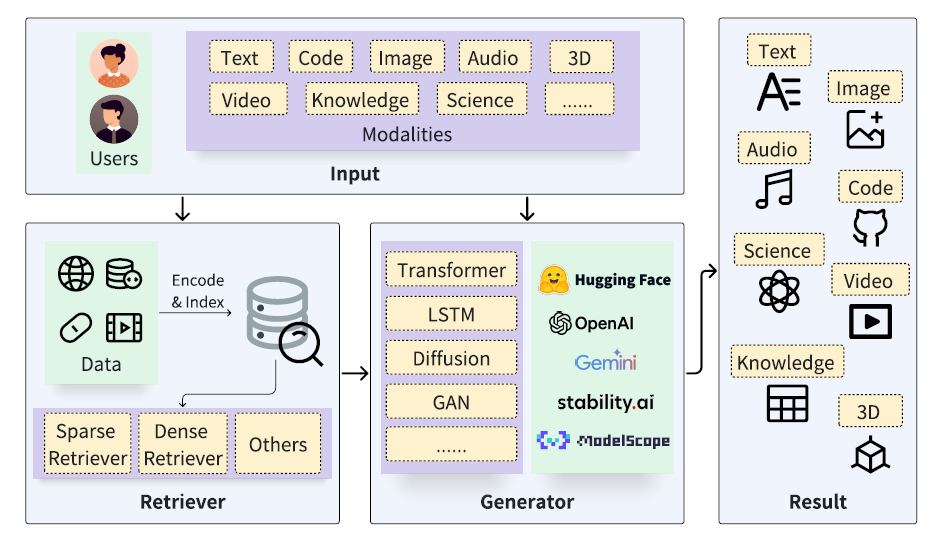
\includegraphics[width=\textwidth]{genericRAGArchitecture.png}
        \caption{Een generieke RAG architectuur \cite{Zhao2024}}
        \label{fig:livebench}
    \end{figure}
    
        \subsubsection{Ophalen}
            \paragraph{Indexeren}
        \subsubsection{Verrijken}
        \subsubsection{Generatie}
    
    
    \subsection{Bouwstenen van RAG}
    
    
        \subsubsection{LLM-modellen voor Retrieval-Augmented Generation (RAG)}
        Welke bestaande LLM-modellen kunnen worden gebruikt voor het ontwikkelen van een Retrieval-Augmented Generation (RAG)? 
        
        %TODO opzoeken wat LLM benchmarks zijn en hoe je ze in deze context kan gebruiken
        
        \paragraph{Introductie}
        Om te bepalen welke modellen het meest geschikt zijn voor de ontwikkeling van een RAG-model, is een objectieve meetmethode noodzakelijk. Gelukkig bestaan er verschillende platforms die LLM's vergelijken en rangschikken op basis van prestaties. In deze sectie bespreken we enkele van deze platforms en maken we een selectie van modellen die het meest geschikt lijken voor het bouwen van een RAG-model.
        
        %TODO overall dieper ingaan hoe ze te werk gaan als het gaat om vergelijken van een LLM dus de paper lezen en samenvatten wat je ermee kan gaan doen
        
        \paragraph{LiveBench} 
        Een platform dat LLM-modellen evalueert, is LiveBench. Dit platform stelt een rangschikking op voor verschillende modellen en biedt een actuele leaderboard die elke zes maanden wordt bijgewerkt. Voor deze bachelorproef zal gebruik worden gemaakt van de ranking afkomstig uit november 2024.
        
        LiveBench beoordeelt LLM-modellen op basis van zes categorieën. Binnen elke categorie worden meerdere taken uitgevoerd om een nauwkeurige beoordeling te verkrijgen. De zes categorieën zijn:
        \begin{itemize}
            \item Wiskundige vaardigheden (Math)
            \item Programmeervaardigheden (Coding)
            \item Redeneren en probleemoplossing (Reasoning)
            \item Data-analyse (Data Analysis)
            \item Volgen van instructies (Instruction Following)
            \item Begrip van natuurlijke taal (Language Comprehension)
        \end{itemize}
        
        Elke categorie wordt geëvalueerd op basis van specifieke taken. Dit resulteert uiteindelijk in een algemene rangschikking, waarin zowel de beste modellen per categorie als het beste presterende model overall worden geïdentificeerd.
        
        \begin{figure}[H]
            \centering
            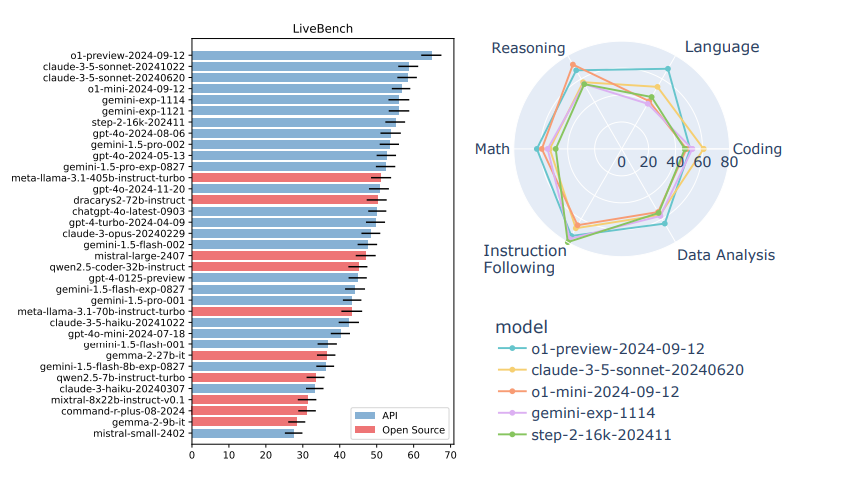
\includegraphics[width=\textwidth]{LiveBenchRanking.png}
            \caption{LiveBench ranking van verschillende LLMs.}
            \label{fig:livebench}
        \end{figure}
        
        \noindent\textbf{Bron:} \textit{LiveBench AI} \url{https://livebench.ai/#/details} (Geraadpleegd op 16 februari 2025).
        
        Uit de ranking van LiveBench kan geconcludeerd worden dat 3 verschillende organisaties elk een model aanbieden die vanuit globaal oogpunt tot de top 3 behoort. Deze top 3 zijn: 
        \begin{enumerate}
            \item claude-3-5-sonnet-20240620 van Anthropic
            \item Meta-llama-3.1-405b-instruct-turbo van Meta
            \item gpt-4o-2024-05-13 van OpenAI
        \end{enumerate}
        
        \subsubsection{Chatbot arena} 
        
        %TODO uitleggen hoe de scoring werkt van chatbot en eventueel uitleggen wat de verschillen zijn met LiveBench, ik denk vooral dat Chatbot arena getest wordt door mensen en zij hun mening op een grote schaal uitdrukken
        Een andere benchmark tool Chatbot arena, net zoals livebench is Chatbot arena een site die een actuele weergave biedt van de beste LLM's op basis van vooraf gedefinieerde catgeoriën. Op het moment van het schrijven van deze literatuurstudie is de top 3 LLM's volgens deze site de volgende:
        
        \begin{enumerate}
            \item GPT-4-Turbo van OpenAI
            \item GPT-4-0613 van OpenAI
            \item Mistral-Medium Mistral AI
        \end{enumerate}
        
        Hoewel het doel van beide benchmarks hetzelfde is is de manier van werken wel anders. ChatbotArena gaat gebruikers twee anonieme LLM modellen tegenover elkaar plaatsen, de gebruiker kan vervolgens een eigen vraag stellen en de gebruiker bepaalt zelf welke van de 2 het beste resultaat heeft opgeleverd.
        
        Het voordeel van deze methode is dat de LLM-modellen realistische cases moeten behandelen die door gebruikers zelf worden gesteld. Op basis van resultaten die de LLM modellen tonen kan een gebruiker zijn voorkeur meegeven. Het nadeel van deze manier van werken is dat de gebruikers die deze testen uitvoeren niet respresentatief zijn voor alle gebruikers van LLM-modellen. De gebruikers die deze testen uitvoeren zijn vaak mensen met een interesse in LLM-modellen of mensen die onderzoek doen in dit vakgebied. Desoondanks kan op basis van deze stemmen verscheidene modellen tegenover elkaar worden geplaatst. In januari 2024 werden ruim 240.000 stemmen uitgebracht door ongeveer 90.000 gebruikers \autocite{Chiang2024}. 
        
        %TODO Hier dit verder uitschrijven, ik denk niet dat je de volgende vraag kan beantwoorden dus ik zou meteen nagaan welke tools, frameworks er zijn die je kan gebruiken.
        
        %TODO zet hier ook de actuele ranking van beide benchmarks. Al was het maar om te duiden dat het een sterk veranderende wereld is waar en dat naar alle waarschijnlijkheid de modellen die nu worden gebruikt waarschijnlijk al achterhaald zullen zijn.
        
        \paragraph{Conclusie}
        Op basis van de 2 benchmarks die hier werden besproken kan niet meteen éénduidig besloten worden welke modellen het best zouden gebruikt worden voor het maken van het RAG model. Aangezien dit een zeer volatiele omgeving is met veel en snelle ontwikkelingen zijn de modellen die vandaag het beste scoren over een maand potentieel voorbij gestoken door nieuwe modellen. Desalniettemin bevatten deze benchmarks heel wat nuttige informatie en inzichten over de sterktes van bepaalde modellen tegenover andere modellen. 
     
    \subsection{RAG voor documentgebaseerde ondersteuning}
    Welke bestaande tools en frameworks kunnen bijdragen aan het opzetten van een RAG?
    
    \subsection{Tools en frameworks voor RAG}
    Welke bestaande tools en frameworks kunnen bijdragen aan het opzetten van een RAG?

\section{De AI Act en de belangrijkste richtlijnen}
Wat houdt de AI Act in, en wat zijn de belangrijkste richtlijnen die hierin moeten worden gevolgd?

\section{Best practices voor IT-supportprocessen}
Wat zijn de bestaande best practices voor de organisatie van IT-supportprocessen?

%%=============================================================================
%% Methodologie
%%=============================================================================

\chapter{\IfLanguageName{dutch}{Methodologie}{Methodology}}%
\label{ch:methodologie}

%% TODO: In dit hoofstuk geef je een korte toelichting over hoe je te werk bent
%% gegaan. Verdeel je onderzoek in grote fasen, en licht in elke fase toe wat
%% de doelstelling was, welke deliverables daar uit gekomen zijn, en welke
%% onderzoeksmethoden je daarbij toegepast hebt. Verantwoord waarom je
%% op deze manier te werk gegaan bent.
%% 
%% Voorbeelden van zulke fasen zijn: literatuurstudie, opstellen van een
%% requirements-analyse, opstellen long-list (bij vergelijkende studie),
%% selectie van geschikte tools (bij vergelijkende studie, "short-list"),
%% opzetten testopstelling/PoC, uitvoeren testen en verzamelen
%% van resultaten, analyse van resultaten, ...
%%
%% !!!!! LET OP !!!!!
%%
%% Het is uitdrukkelijk NIET de bedoeling dat je het grootste deel van de corpus
%% van je bachelorproef in dit hoofstuk verwerkt! Dit hoofdstuk is eerder een
%% kort overzicht van je plan van aanpak.
%%
%% Maak voor elke fase (behalve het literatuuronderzoek) een NIEUW HOOFDSTUK aan
%% en geef het een gepaste titel.


\section{Literatuurstudie}
Voor de opstart van deze bachelorproef is een uitgebreide literatuurstudie essentieel om de bestaande mogelijkheden op het gebied van virtuele assistenten te verkennen. Deze studie richt zich op een vergelijkende analyse die inzicht biedt in de verschillende beschikbare opties voor het ontwikkelen van een virtuele supportassistent. Hierbij worden de voor- en nadelen van elke optie in kaart gebracht, zodat op basis van deze informatie een onderbouwde keuze kan worden gemaakt voor de uitwerking van een PoC. De literatuurstudie moet ook duidelijkheid verschaffen over de benodigde hardware- en softwarevereisten voor de ontwikkeling.

Op basis van de literatuurstudie moet een analyse worden opgesteld om na te gaan welke optie die werden besproken binnen de literatuurstudie het best in overweging worden genomen. De belangrijkste keuze die zal moeten gemaakt worden binnen deze use case is de keuze tussen een RAG implementatie of een CAG implementatie. Aangezien beide voor- en nadelen hebben moet dit weloverwogen worden voor het opstellen van de PoC en het LLM modellen die kunnen worden gebruikt voor de PoC.


\section{Requirement analyse}


Gekoppeld aan de literatuurstudie zullen interviews worden afgenomen. Het doel van deze interviews is om een helder overzicht te verkrijgen van de verschillende vereisten voor de virtuele assistent. Op basis van het overzicht uit de literatuurstudie kan vervolgens een meer gerichte selectie worden gemaakt van de verschillende opties. Het uiteindelijke doel is om voor twee à drie modellen een PoC uit te werken die verder getest kunnen worden. Het is met andere woorden van belang om de verschillende modellen zo uitgebreid mogelijk te onderzoeken, zodat zoveel mogelijk modellen getoetst kunnen worden aan de gevraagde vereisten.Eens de literatuurstudie is afgerond en de interviews zijn afgenomen, kan met behulp van een MoSCoW-analyse een rangschikking worden opgesteld van de verschillende beschikbare modellen. Deze rangschikking bepaalt welke modellen worden geselecteerd voor het uitwerken van een PoC.

\section{Long list}

\section{Short list}

\section{Opstellen PoC}

\section{Uitvoeren testen en analyse resultaten}

Elk van de geselecteerde modellen wordt vervolgens uitgewerkt in een PoC. Zodra de verschillende PoC’s beschikbaar zijn, wordt een vergelijking gemaakt tussen de modellen. Hierbij worden de volgende aspecten specifiek getest:

\begin{itemize} 
    \item Wat is de kwaliteit van de antwoorden? 
    \item Wat is de tijd en de kost van een query?
    \item Hoe eenvoudig is het om het model op te zetten? 
\end{itemize}

De kwaliteit van de antwoorden zal worden gemeten aan de hand van de ROUGE-score, terwijl de tijd per query gemeten en vergeleken zal worden per model. Gezien het derde criterium eerder subjectief is, zal dit minder doorwegen in de uiteindelijke vergelijking. Aan de hand van deze drie criteria zal uiteindelijk een vergelijking worden gemaakt, waaruit zal blijken welk model het beste voldoet aan de gevraagde functionaliteit. Zo kan aan het einde van het onderzoek worden bepaald welke van de verschillende PoC's de meeste troeven heeft om in de praktijk te worden gebruikt.




% Voeg hier je eigen hoofdstukken toe die de ``corpus'' van je bachelorproef
% vormen. De structuur en titels hangen af van je eigen onderzoek. Je kan bv.
% elke fase in je onderzoek in een apart hoofdstuk bespreken.

%%=============================================================================
%% Proof of concept
%%=============================================================================
\chapter{Proof of concept}
\label{ch:proof-of-concept}
%TODO cpations bij figuren nakijken

%Wat wil je bewijzen of aantonen met deze PoC?
De hoofddoelstelling van deze PoC is te onderzoeken hoe een LLM ondersteuning kan bieden binnen een IT-supportsysteem, met als doel technische IT-vragen sneller af te handelen. De toepassing is bedoeld voor intern gebruik door het IT-team en niet voor externe gebruikers, zoals burgers. Verschillende benaderingen werden onderzocht, waaruit bleek dat RAG de meest geschikte methode is voor deze context.
\\[1em]
%Welke hypothese test je eigenlijk?
De hypothese die binnen deze PoC getest wordt, kan als volgt worden samengevat:
\textit{“Een LLM, gecombineerd met Retrieval-Augmented Generation (RAG), kan effectief en efficiënt ondersteuning bieden binnen een IT-supportsysteem door relevante informatie uit documentatie te halen en daarmee het supportproces te optimaliseren en te vereenvoudigen.”}

\section{Behoeften analyse}
Voor de PoC werd een MoSCoW-analyse uitgevoerd om de functionele vereisten te prioritiseren.
De analyse werd onderverdeeld in \textit{Must haves}, \textit{Should haves} en \textit{Could haves}

\subsection{Must haves}
\begin{itemize}
    \item \textbf{Vragen kunnen stellen in de eigen taal (bijvoorbeeld Nederlands, Frans of Engels)}:\\ 
    Het systeem moet correct functioneren ongeacht of de gebruiker vragen stelt in het Nederlands, Frans of Engels.
    \item \textbf{Een duidelijk en bruikbaar antwoord ontvangen op basis van betrouwbare bronnen}:\\ 
    De gegenereerde antwoorden moeten informatief, relevant en praktisch toepasbaar zijn.
    \item \textbf{Eenvoudige en intuïtieve interface}:\\  
    De gebruiker mag geen technische kennis nodig hebben. De interactie moet vanzelfsprekend en gebruiksvriendelijk aanvoelen.
    \item \textbf{Consistente ervaring (snel, zonder fouten of willekeurige antwoorden)}:\\  
    De gebruiker verwacht dat de applicatie betrouwbaar functioneert en consistente resultaten levert.
\end{itemize}

\subsection{Should haves}
\begin{itemize}
    \item \textbf{Het systeem begrijpt vervolgvragen binnen een sessie}:\\  
    De gebruiker moet een gesprek kunnen voeren waarbij eerdere vragen worden meegenomen in de context, zodat interacties natuurlijker verlopen.
    \item \textbf{Transparantie over de gebruikte bronnen van het antwoord}:\\  
    De gebruiker moet kunnen zien uit welk document of welke bron het antwoord afkomstig is, zodat de informatie steeds gecontroleerd en gevalideerd kan worden.
\end{itemize}

\subsection{Could haves}
\begin{itemize}
    \item \textbf{Langetermijngeheugen over meerdere sessies heen}:\\  
    Het opzetten van een geheugen dat sessie-overstijgend werkt, brengt extra complexiteit met zich mee en is daarom minder geschikt voor een eerste versie.
    \item \textbf{Zelf documenten kunnen uploaden of bewerken}:\\  
    In deze PoC ligt de focus op het zoeken en beantwoorden van vragen, niet op het beheren van documenten.
    \item \textbf{Automatisch mails behandelen}:\\  
    Het automatisch verwerken en beantwoorden van e-mails valt qua complexiteit buiten de scope van een eerste versie.
\end{itemize}

\section{Architectuur en Ontwerp}

Vooraleer de structuur van de PoC kan worden opgezet, moet er een keuze gemaakt worden voor de meest geschikte techniek. Finetuning is, gelet op de scope van de PoC, moeilijk uitvoerbaar. Om dit te realiseren zou een model getraind moeten worden op data die kan helpen bij IT-support. Hoewel er data beschikbaar is in de vorm van e-mails, is het onderhoud bij finetuning niet te onderschatten. Wanneer een procedure of gegevens veranderen, moet het model immers opnieuw getraind worden. Deze keuze brengt met andere woorden een hoge initiële kost met zich mee en potentieel ook een hogere onderhoudskost, die niet aanwezig is bij RAG of CAG.
\\[1em]
Met CAG aan de andere kant zouden alle documenten worden toegevoegd aan de context. Hoewel dit technisch mogelijk is, zeker met de modellen van vandaag, heeft deze aanpak enkele nadelen. Ten eerste kan \textit{context rot} een probleem vormen. Zoals aangegeven in de stand van zaken, worden modellen minder performant wanneer te veel informatie in de context wordt geplaatst. Daarnaast wordt bij CAG niet alleen relevante, maar ook irrelevante informatie toegevoegd. Dit verhoogt niet alleen de kans op minder nauwkeurige antwoorden, maar ook de mogelijke API-kosten in vergelijking met RAG.
\\[1em]
Met al deze redenen in gedachten is voor deze PoC gekozen om RAG toe te passen. Enerzijds zijn er geen hoge initiële kosten zoals bij finetuning, en anderzijds worden enkel relevante documenten toegevoegd aan de context. Dit helpt om mogelijke problemen van context rot te vermijden en houdt bovendien de kost per query laag. Tabel \ref{tab:techniek_vergelijking} geeft een overzicht van de voor- en nadelen van de verschillende benaderingen.

\begin{table}[H]
    \resizebox{\textwidth}{!}{
            \begin{tabular}{|p{4cm}|c|c|c|}
            \hline
            \textbf{Kenmerk} & \textbf{Finetuning} & \textbf{CAG} & \textbf{RAG} \\
            \hline
            Initiële kost & Hoog & Laag & Laag \\
            \hline
            Onderhoudskost & Hoog & Laag & Laag \\
            \hline
            Document selectie & n.v.t -- kennis zit in model & Alle documenten & Enkel relevante \\
            \hline
            Kost per query & Laag & Potentieel hoog  & Laag \\
            \hline
            Implementatie & Complex door training model & Relatief eenvoudig & Complex door implementatie retrieval\\
            \hline
        \end{tabular}
    }
    \caption{Vergelijking van voor- en nadelen van finetuning, CAG en RAG}
    \label{tab:techniek_vergelijking}
\end{table}

\subsection{Algemene structuur}

Deze structuur bestaat uit een graaf die is opgebouwd uit verschillende knooppunten (nodes). De graaf stelt het LLM bovendien in staat om zelfstandig te bepalen welke keuzes gemaakt moeten worden tijdens het verwerken van een vraag.
\\[1em]
De standaard RAG-architectuur gaat een query gaan embedden en haalt vervolgens de meest relevante documenten op uit de vectordatabase, zonder verdere reflectie over de nood van het ophalen van de documenten en de werkelijke relevantie van deze documenten. Hoewel dit op het eerste gezicht een efficiënte aanpak lijkt, betekent het ook dat het systeem bij elke willekeurige gebruikersvraag opnieuw de vectordatabase bevraagt, zelfs wanneer dat niet noodzakelijk is.
\\[1em]
Om dit te vermijden, werd gebruikgemaakt van een graafstructuur die de LLM de mogelijkheid geeft om zelf te beoordelen wanneer het relevant is om documenten op te halen. Daarnaast wordt de LLM ook verantwoordelijk geacht om te oordelen over de opgehaalde documenten. De volledige flow van het proces kan worden bekeken in figuur~\ref{fig:Architectuur}
\\[1em]
De PoC werd uitgewerkt met behulp van Ollama, een tool waarmee open modellen lokaal kunnen worden gedraaid. Tijdens overleg met de betrokken partijen werd geen voorkeur uitgesproken voor specifieke LLM-modellen, enkel het gebruik van DeepSeek werd afgeraden.

\begin{figure}[H]
    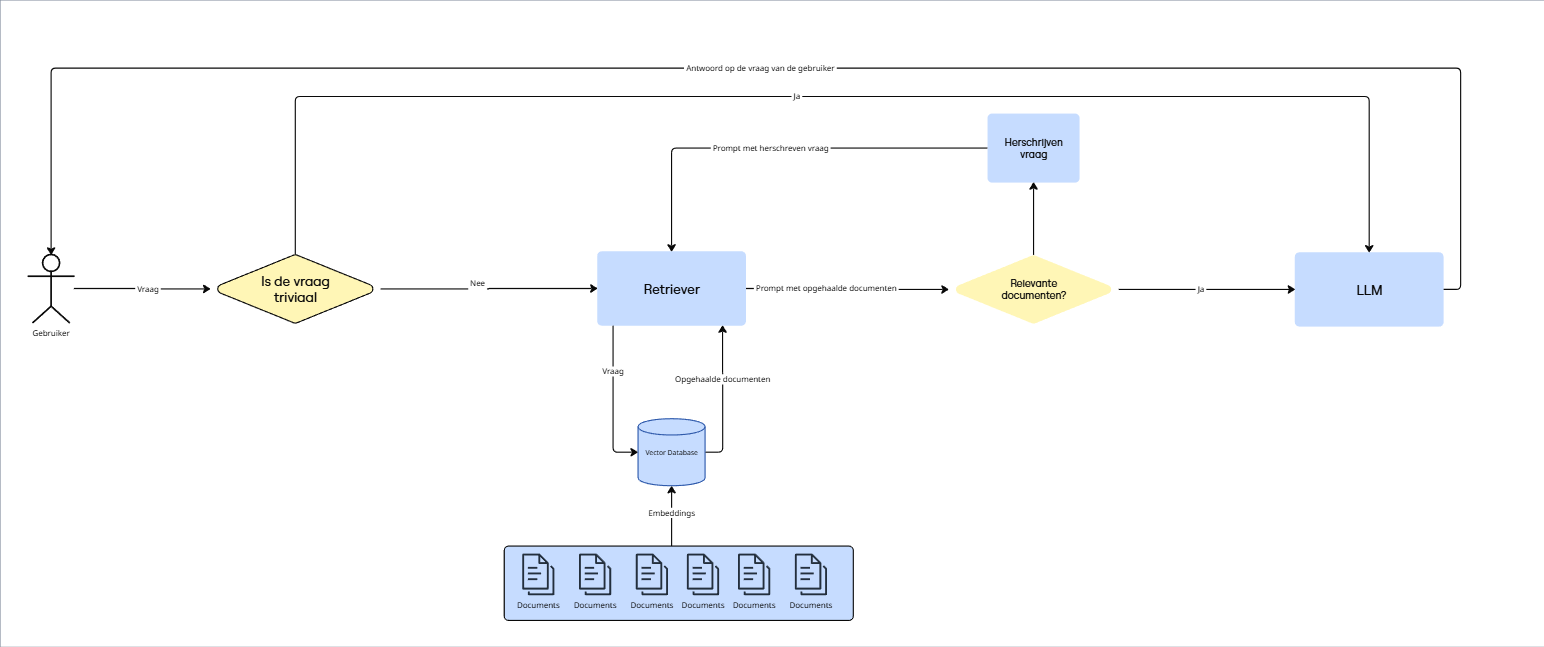
\includegraphics[width=1\textwidth]{flowchart.png}
    \caption{Architectuur van de PoC op basis van een graafgebaseerde workflow}
    \label{fig:Architectuur}
\end{figure}

%Belangrijke keuzes tijdens het bouwen (waarom bv. technologie X en niet Y?).

Een van de belangrijkste beslissingen in deze PoC was de initiële keuze voor RAG ten opzichte van andere mogelijke benaderingen. Eens deze keuze gemaakt was, volgde de selectie van een geschikt framework om RAG te implementeren.
\\[1em]
Voor deze PoC werd gekozen voor LangGraph, een framework waarmee zogenaamde agents kunnen worden opgebouwd aan de hand van grafen. Dit verschilt van bijvoorbeeld LangChain, waar gewerkt wordt met ketens van opeenvolgende stappen.
\\[1em]
LangGraph biedt meer flexibiliteit in het aansturen van de flow en logica binnen het systeem. Zo kan een LLM bijvoorbeeld zelf kiezen welke paden in de graaf doorlopen worden, of kan er een lus geïntroduceerd worden binnen de graafstructuur. Beide mechanismen werden effectief toegepast in deze PoC.
\\[1em]
%Qwen3 hypoImage vraag zie je rewrite en 2de poging lukt het wel
Dit is bijzonder nuttig in deze use case omdat er voldaan moet worden aan een meertalige omgeving. Het is vooraf namelijk niet zeker in welke taal de gebruiker de toepassing zal gebruiken. Dit kan Frans, Nederlands of Engels zijn. Daarnaast is de documentatie zelf ook in verschillende talen beschikbaar. Met andere woorden kan een vraag in het Nederlands gesteld worden terwijl de documentatie enkel in het Frans beschikbaar is, wat soms tot problemen leidt in het retrievalproces. Door te werken met een graaf kan de LLM complexere paden volgen die bijvoorbeeld met LangChain niet mogelijk zouden zijn geweest.
\\[1em]
Daarnaast maakt deze aanpak het mogelijk om de capaciteiten van verschillende modellen te testen. Het is immers aan het LLM-model zelf om op verschillende momenten in het proces keuzes en inschattingen te maken.

\subsection{Gebruikte tools en frameworks}
Hieronder een overzicht van de verschillende frameworks, tools en programmeertalen die werden gebruikt om deze PoC op te stellen.

\begin{table}[H]
    \begin{tabular}{|l|l|}
        \hline
        \textbf{Categorie}       & \textbf{Technologieën}               \\ \hline
        Frameworks/Libraries     & LangChain, LangGraph, Streamlit, Ragas \\ \hline
        Tools                   & ChromaDB, Ollama                    \\ \hline
        Programmeertalen        & Python                             \\ \hline
    \end{tabular}
    \caption{Overzicht van de gebruikte technologieën}
\end{table}

%Schema’s (bv. systeemdiagram, flowchart) zijn hier heel sterk.

\section{Implementatie}

%Hoe heb je de POC concreet opgebouwd?

\subsection{vectorstore}
De PoC werd opgebouwd volgens de klassieke RAG-implementatie. In de eerste fase werden de originele documenten opgesplitst in kleinere tekstsegmenten en vervolgens omgezet naar embeddings via een vooraf getraind embedding model. Voor deze PoC werd hiervoor gebruikgemaakt van het \verb|mxbai-embed-large model|. Van de beschikbare embedding modellen binnen Ollama biedt dit model de hoogste semantische nauwkeurigheid.

\begin{lstlisting}[basicstyle=\small, frame=single, breaklines=true, postbreak=\mbox{\textcolor{red}{$\hookrightarrow$}\space}, escapeinside ={\%,}, escapechar={!}, numbers=left, language=Python, caption=Ophalen van embedding model]
def get_embedding():
    return OllamaEmbeddings(model='mxbai-embed-large')
\end{lstlisting}

Gekoppeld aan het embedding model is er ook een chatmodel dat doorheen het proces wordt gebruikt. De variabele \verb|response_model_name| bepaalt welk model wordt gebruikt tijdens de flow. De enige configuratie die werd aangepast, is het instellen van de temperatuur op nul. De temperatuur bepaalt hoe creatief het model zal zijn in zijn antwoorden. Aangezien het de bedoeling is om zo weinig mogelijk hallucinaties te veroorzaken, werd ervoor gekozen om deze waarde op nul te zetten. Welke modellen zijn gekozen en waarom, wordt in een latere sectie besproken.

\begin{lstlisting}[basicstyle=\small, frame=single, breaklines=true, postbreak=\mbox{\textcolor{red}{$\hookrightarrow$}\space}, escapeinside ={\%,}, escapechar={!},
numbers=left, language=Python, caption=Initialisatie van het chat model]
def get_response_model():
    return ChatOllama(model=response_model_name, temperature=0)
\end{lstlisting}

\subsubsection{Opbouw vector database}
Om de vector database op te bouwen, wordt één functie gebruikt. De volledige functie is voor de volledigheid toegevoegd als bijlage \ref{functie-vectorstore}.
\\[1em]
De functie bevat verschillende parameters die nodig zijn voor het opbouwen van de vectorstore. Ten eerste is er de embeddings functie die zojuist besproken is, vervolgens de locatie waar de documenten beschikbaar zijn, daarna de naam van de database en tot slot de laatste twee parameters die worden gebruikt om in te stellen hoe er gezocht moet worden in de database. Dit hangt af van de gekozen ophaalmethode.

\begin{lstlisting}[basicstyle=\small, frame=single, breaklines=true, postbreak=\mbox{\textcolor{red}{$\hookrightarrow$}\space}, escapeinside ={\%,}, escapechar={!},
    numbers=left, language=Python, caption=Functie met parameters]
def build_vector_store(embeddings_function, document_path, db_name, search_type, search_kwargs):
\end{lstlisting}

Gebruik makend van onderstaande dictionary wordt een loader geselecteerd die in een latere fase wordt gebruikt om de documenten te parsen.

\begin{lstlisting}[basicstyle=\small, frame=single, breaklines=true, postbreak=\mbox{\textcolor{red}{$\hookrightarrow$}\space}, escapeinside ={\%,}, escapechar={!},
    numbers=left, language=Python, caption=Mapping van bestandsextensies naar de bijbehorende document loaders]
loader_mapping = {
    ".md": TextLoader,
    ".txt": TextLoader,
    ".pdf": PyPDFLoader,
    ".docx": UnstructuredWordDocumentLoader,
    ".doc": UnstructuredWordDocumentLoader,
}
\end{lstlisting}

In het onderstaande codefragment worden de documenten ingelezen en verzameld in een array. De inhoud wordt, afhankelijk van de extensie, met een specifieke loader ingelezen. Elk document krijgt extra metadata mee, namelijk de map en het pad naar het bestand, zodat later duidelijk is om welk document het gaat.

\begin{lstlisting}[basicstyle=\small, frame=single, breaklines=true, postbreak=\mbox{\textcolor{red}{$\hookrightarrow$}\space}, escapeinside ={\%,}, escapechar={!},
    numbers=left, language=Python, caption=Inladen en parsen van documenten per bestandstype met toevoeging van metadata]
    documents = []
    for doc_file_path in glob.glob(os.path.join(folder, f"*{ext}")):
        try:
            document = base_loader_type(doc_file_path, encoding="utf-8")
            doc = document.load()
            for d in doc:
                d.metadata = {"source": doc_file_path, "folder": folder}
                documents.append(d)
        except Exception as e:
            print(f"Failed to load file {doc_file_path}: {e}")
\end{lstlisting}

Hierna worden de documenten opgesplitst in chunks. Elke chunk heeft een grootte van 2000 karakters, met een overlap van 500 karakters tussen opeenvolgende chunks. Na het testen van verschillende chunk groottes bleek dit de kleinst mogelijke waarde te zijn waarbij nog voldoende relevante informatie kon worden opgehaald.

\begin{lstlisting}[basicstyle=\small, frame=single, breaklines=true, postbreak=\mbox{\textcolor{red}{$\hookrightarrow$}\space}, escapeinside ={\%,}, escapechar={!}, numbers=left, language=Python, caption=Vector store build] 
# Split the document into chunks
text_splitter = RecursiveCharacterTextSplitter(chunk_size=2000, chunk_overlap=500)
docs = text_splitter.split_documents(documents)
\end{lstlisting}

De gegenereerde embeddings worden vervolgens opgeslagen in een vectorstore. Voor deze PoC is gekozen voor ChromaDB, een performante en gebruiksvriendelijke oplossing. Hoewel alternatieven zoals FAISS eveneens mogelijk zijn, is de keuze gevallen op ChromaDB vanwege de uitgebreide documentatie en de brede ondersteuning binnen het gebruikte framework LangGraph. Hierdoor kon de implementatie op een efficiënte worden uitgevoerd.

\begin{lstlisting}[basicstyle=\small, frame=single, breaklines=true, postbreak=\mbox{\textcolor{red}{$\hookrightarrow$}\space}, escapeinside ={\%,}, escapechar={!}, numbers=left, language=Python, caption=Vector store build]
# Return a ChromaDB instance
return (Chroma.from_documents(
        docs, embeddings_function, persist_directory=persistent_directory)
        .as_retriever(search_type=search_type, search_kwargs=search_kwargs))
\end{lstlisting}

Deze initiële set-up maakt het mogelijk om relevante documenten snel op te halen op basis van semantische gelijkenis met de vraag van de gebruiker. Met andere woorden: dit vormt een kerncomponent van de RAG-oplossing.

\subsection{Graaf structuur en nodes}

Eens de vector met de nodige documenten beschikbaar is kunnen er vragen gesteld worden aan de LLM die aan de hand van een graaf keuzes zal maken naargelang de vraag van de gestelde gebruiker. De volledige workflow werd gemodelleerd als een LangGraph-graaf. Deze structuur is weergegeven in figuur~\ref{fig:langgraph}.

\begin{figure}[H]
    \centering
    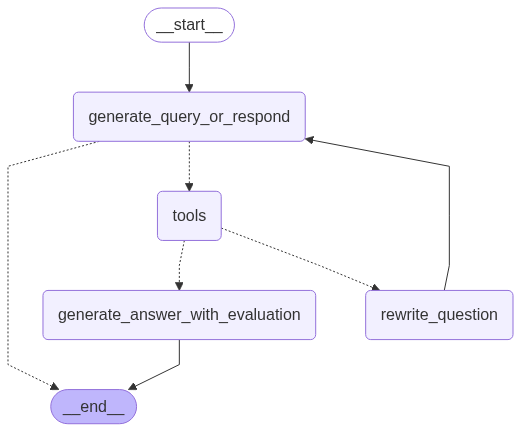
\includegraphics[width=0.8\textwidth]{langgraph_workflow.png}
    \caption{Technische uitwerking van de workflow als LangGraph-graaf}
    \label{fig:langgraph}
\end{figure}

\subsubsection{Antwoorden of documenten ophalen}

Vooraleer het RAG-proces op gang wordt gebracht, moet de LLM eerst een inschatting maken van de vraag die de gebruiker heeft gesteld. Wanneer het gaat om een triviale vraag of een eenvoudig bericht, dient de LLM onmiddellijk een antwoord te geven, zonder het volledige RAG-proces te doorlopen.
\\[1em]
Om dit te realiseren, wordt gebruikgemaakt van de volgende prompt, waarin de input van de gebruiker wordt ingevuld: 

\begin{lstlisting}[basicstyle=\small, frame=single, breaklines=true, postbreak=\mbox{\textcolor{red}{$\hookrightarrow$}\space}, escapeinside ={\%,}, escapechar={!}, numbers=left, language=Python, caption=Prompt voor beslissen tussen direct antwoord of documentopvraging]
RETRIEVE_DOCUMENTS_OR_RESPOND_PROMPT = """
    This method decides whether to call the retriever tool or respond directly.
    
    If the user's question is trivial, respond directly. Just respond directly. Do not show your reasoning or thinking process.
    If the question is non-trivial, use the retriever tool to generate a response.
    If in doubt, use the retriever tool to make sure.
    
    Given the user's question:  
    "{message}"
    
    Determine whether the question is trivial. 
"""
\end{lstlisting}

Het voordeel van deze aanpak is dat er geen onnodige resources worden verbruikt bij het uitvoeren van het RAG-proces. Enkel wanneer de vraag van de gebruiker effectief nood heeft aan specifieke contextuele informatie, wordt de retriever geactiveerd.
\\[1em]
De LLM krijgt een retriever tool ter beschikking en kan vervolgens autonoom beslissen of deze tool wordt gebruikt of dat er meteen een antwoord gegenereerd wordt. Dit gedrag wordt geïmplementeerd in de volgende node:

\begin{lstlisting}[basicstyle=\small, frame=single, breaklines=true, postbreak=\mbox{\textcolor{red}{$\hookrightarrow$}\space}, escapeinside ={\%,}, escapechar={!}, numbers=left, language=Python, caption=Functie die beslist tussen direct antwoord en documentopvraging]
def retrieve_documents_or_respond(state: MessagesState) -> MessagesState:
    """
    This methods will call the retriever tool when given a non trivial question is asked.
    In the case of a trivial question it will simply provide a response
    Call the model to generate a response based on the current state. Given
    the question, it will decide to retrieve using the retriever tool, or simply respond to the user.
    """
    message = state["messages"][-1].content
    
    prompt = RETRIEVE_DOCUMENTS_OR_RESPOND_PROMPT.format(message=message)
    
    response_model_with_tools = response_model.bind_tools([myminfin_retriever_tool])
    response = response_model_with_tools.invoke([SystemMessage(content=prompt),
    HumanMessage(content=message)])
    return MessagesState(messages=[response])
\end{lstlisting}

In deze stap ontvangt de LLM twee afzonderlijke berichttypes, een SystemMessage en een HumanMessage.
\\[1em]
De SystemMessage bevat instructies voor het model over hoe het dient te handelen. De oorspronkelijke gebruikersvraag wordt hierbij in de prompt (RETRIEVE\_DOCUMENTS\_OR\_RESPOND\_PROMPT) geïntegreerd, zodat de LLM beschikt over context en richtlijnen voor de verdere verwerking.
\\[1em]
Daarnaast wordt de gebruikersvraag ook afzonderlijk toegevoegd als een HumanMessage. Dit berichttype geeft expliciet aan dat de inhoud afkomstig is van een menselijke gebruiker.
\\[1em]
Uit eerdere tests is gebleken dat het opnemen van beide berichttypes noodzakelijk is om optimale resultaten te behalen. De SystemMessage verschaft duidelijke instructies en context, terwijl de HumanMessage de oorspronkelijke vraag onvervormd aan het model doorgeeft. Op deze manier beschikt het model zowel over specifieke richtlijnen en het exacte bericht van de gebruiker, wat de kans op correcte interpretatie en verwerking vergroot.

\subsubsection{Retriever}

Zodra de keuze wordt gemaakt om documenten op te halen, roept het LLM-model de retriever-tool aan. Deze tool raadpleegt ChromaDB om, op basis van een vooraf bepaalde retrieval methode, de relevante documenten op te halen. Er zijn verschillende methoden beschikbaar om tekstfragmenten (chunks) uit de vectordatabank op te vragen. Na het testen van meerdere opties werd gekozen voor de \verb|similarity search| methode.
\\[1em]
De alternatieve ophaal methoden bleken minder geschikte resultaten op te leveren. Het eerste alternatief, \verb|similarity_score_threshold|, vertoont overeenkomsten met de gebruikte \verb|similarity search|, in de zin dat eveneens de meest relevante documenten worden opgehaald. Het verschil is dat bij deze aanpak een vooraf ingestelde relevantie drempelwaarde vereist is. Alleen chunks die voldoen aan deze drempel worden uit de vector database opgehaald. In de praktijk leidde dit ertoe dat bij bepaalde vragen geen enkele chunk als relevant werd beschouwd, waardoor de vraag niet kon worden beantwoord, ondanks dat het antwoord wel aanwezig was in de vector database.  
\\[1em]
Het tweede alternatief, \textit{Maximal Marginal Relevance} (MMR), kiest daarentegen bewust voor zo veel mogelijk variatie in de opgehaalde chunks. Dit resulteerde echter vaak in documenten die onvoldoende relevant waren ten opzichte van de gestelde vraag.  
\\[1em]
Om die redenen werd uiteindelijk gekozen voor de \verb|similarity search| methode. Deze benadering selecteert de documenten die het meest relevant zijn voor de vraag. In deze PoC specifiek worden bij elke bevraging de vier meest relevante documenten uit de vector database opgehaald.

\subsubsection{Beoordeling documenten}

Na het ophalen van de documenten moet de LLM opnieuw evalueren of het over voldoende informatie beschikt om een antwoord te formuleren. Indien de documenten voldoende relevantie vertonen ten opzichte van de oorspronkelijke vraag, wordt overgegaan tot het genereren van een antwoord. Indien dit niet het geval is, zal de oorspronkelijke vraag geherformuleerd worden en wordt het ophaal proces opnieuw opgestart.

\begin{lstlisting}[basicstyle=\small, frame=single, breaklines=true, postbreak=\mbox{\textcolor{red}{$\hookrightarrow$}\space}, escapeinside ={\%,}, escapechar={!}, numbers=left, language=Python, caption=Functie die beslist tussen antwoord genereren of vraag herschrijven]
def grade_documents(
state: MessagesState,
) -> Literal["generate_answer", "rewrite_question"]:
    """Determine whether the retrieved documents are relevant to the question."""
    
    # Shortcut: If too many messages (multiple rewrites), stop rewriting
    if len(state["messages"]) >= 5:
    return "generate_answer"
    
    question = state["messages"][0].content
    context = state["messages"][-1].content
    
    prompt = GRADE_DOCUMENTS_PROMPT.format(question=question, context=context)
    response = (
    grader_model
        .with_structured_output(GradeDocuments)
        .invoke([HumanMessage(content=prompt)])
    )
    score = response.binary_score
    
    if score == "yes":
        return "generate_answer"
    else:
        return "rewrite_question"
\end{lstlisting}

Om te vermijden dat de LLM de initiële vraag eindeloos blijft herformuleren, wordt gecontroleerd hoe lang de array van de MessagesState is. Wanneer het aantal berichten gelijk is aan of groter is dan 5 (wat neerkomt op maximaal twee herformuleringen), wordt het model verplicht om door te gaan naar de node die verantwoordelijk is voor het genereren van een antwoord. Op die manier wordt gegarandeerd dat de gebruiker binnen een beperkt aantal stappen een antwoord ontvangt.
\\[1em]
Om ervoor te zorgen dat de LLM deze vraag op een correcte manier gaat verwerken worden zowel de opgehaalde documenten als de originele vraag in een prompt toegevoegd. Hierna is het aan de LLM om een oordeel te vellen over de opgehaalde documenten en de mate waarin deze relevant en nuttig zijn om een vraag te beantwoorden.
\begin{lstlisting}[basicstyle=\small, frame=single, breaklines=true, postbreak=\mbox{\textcolor{red}{$\hookrightarrow$}\space}, escapeinside ={\%,}, escapechar={!}, numbers=left, language=Python, caption=Prompt om opgehaalde documenten te beoordelen op basis van de gestelde vraag]
GRADE_DOCUMENTS_PROMPT = (
    "You are a grader assessing relevance of a retrieved document to a user question. \n "
    "Here are the retrieved documents: \n\n {context} \n\n"
    "Here is the user question: {question} \n"
    "If the document contains keyword(s) or semantic meaning related to the user question, grade it as relevant. \n"
    "Give a binary score 'yes' or 'no' score to indicate whether the document is relevant to the question."
)
\end{lstlisting}

\subsubsection{Genereren antwoord}

Wanneer het hele proces doorlopen is moet de LLM aan de slag met de opgehaalde documenten en de vraag van de gebruiker. Het is hierbij de bedoeling dat geformuleerd worden in de taal waarin ze origineel werden gesteld, zelfs wanneer de LLM de vraag heeft herschreven. En er geen hallucinaties optreden, wanneer op het einde van het proces de documentatie onvoldoende informatie verschaft over de gestelde vraag moet de LLM dit ook melden aan de gebruiker. Om dit te bewerkstelligen werd de volgende prompt gebruikt: 

\begin{lstlisting}[basicstyle=\small, frame=single, breaklines=true, postbreak=\mbox{\textcolor{red}{$\hookrightarrow$}\space}, escapeinside ={\%,}, escapechar={!}, numbers=left, language=Python, caption=Prompt voor genereren van antwoord op basis van de opgehaalde context]
GENERATE_ANSWER_PROMPT = (
    "You are a helpful assistant supporting users with their MyMinfin IT-related questions.\n"
    "Based on the following context, please provide a clear and complete answer.\n"
    "If the answer is not available in the context, kindly let the user know that you don't have enough information.\n"
    "If the context contains a source, always mention it in your answer as the reference.\n"
    "Always respond in the same language this question {question} is asked, even if the context is in a different language.\n"
    "Do not use Markdown or any special formatting in your answer, respond in plain text only.\n\n"
    "Question: {question}\n"
    "Context: {context}"
)
\end{lstlisting}

\subsection{LLM-model}

Nu er een duidelijk beeld is geschetst van de structuur van de graaf, kan worden bekeken welke modellen in aanmerking komen voor gebruik. Hierbij gelden enkele beperkingen. Ten eerste wordt gebruikgemaakt van zogenoemde open modellen. Dit zijn modellen die lokaal kunnen draaien en gratis te gebruiken zijn. Een tweede, hieraan gerelateerde beperking, zijn de hardwarebeperkingen waarmee deze PoC wordt uitgevoerd. Omdat de modellen lokaal draaien, is het niet mogelijk modellen te gebruiken die meer RAM vereisen dan op het lokale systeem beschikbaar is. Concreet betekent dit dat alleen modellen met maximaal acht miljard parameters in aanmerking komen. Tot slot moeten de modellen in staat zijn toolcalls uit te voeren. Op basis van deze voorwaarden en de rankings op Hugging Face is de volgende lijst met mogelijke modellen opgesteld:

\begin{itemize}
    \item llama-3.1-8b-instruct
    \item llama-3.2
    \item Mistral-7b-instruct
    \item Qwen2.5-7B instruct
    \item smollm2-1.7b-instruct
    \item granite-3.2-8b-instruct
    \item granite-3.3
    \item Qwen3
\end{itemize}

Tijdens het testen van de PoC werden echter enkele problemen vastgesteld met de toolcalls. Dit leidde ertoe dat een aantal modellen niet langer gebruikt kon worden. Dit wordt verder toegelicht in \ref{tool-calls}.

\begin{itemize}
    \item Mistral-7b-instruct
    \item smollm2-1.7b-instruct
    \item granite-3.2-8b-instruct
    \item granite-3.3
\end{itemize}

Aangezien de bovenstaande modellen niet langer bruikbaar bleken, is ervoor gekozen om voor de PoC en de vergelijkende studie de volgende modellen te gebruiken:

\begin{itemize}
    \item llama-3.1-8b-instruct
    \item llama-3.2
    \item Qwen2.5-7B instruct
    \item Qwen3
\end{itemize}


\section{Problemen en oplossingen}

Tijdens de ontwikkeling van de toepassing deden zich verschillende problemen voor. Zo waren er uitdagingen bij het efficiënt parsen van documenten, het uitvoeren van tool calls en het onverwachte gedrag van de LLM bij het werken met een graafstructuur. Voor elk van deze problemen werd een passende oplossing gezocht en geïmplementeerd.

%Waar liep je tegenaan tijdens de implementatie?
\subsection{Document parsing}
Het parsen van documenten naar embeddings bleek een uitdagend proces. PDF-bestanden leverden niet altijd het gewenste resultaat op, en hetzelfde gold voor Word-documenten. De moeilijkheden deden zich vooral voor bij documenten met ongestructureerde elementen. Zo ging bij documenten met tabellen de structuur na het parsen vaak verloren.
\\[1em]
Een goede parsing is echter cruciaal voor een goed functionerende RAG-oplossing. Wanneer documenten niet correct gestructureerd zijn en in die vorm als embeddings worden opgeslagen in de vectordatabase, wordt die gebrekkige structuur mogelijk opnieuw toegevoegd aan de context die de LLM gebruikt. Dit kan leiden tot problemen bij het genereren van kwalitatieve antwoorden.
\\[1em]
Om dit probleem te verhelpen, werden de documenten in een eerste fase omgezet naar docx-bestanden. Aangezien dit eveneens niet het gewenste resultaat opleverde, werd uiteindelijk gekozen om de documenten te converteren naar Markdown formaat. Deze aanpak had als voordeel dat de documentstructuur tijdens het parsen beter behouden bleef. Dit resulteerde in beter gestructureerde, relevante chunks die vervolgens als context konden worden gebruikt bij het beantwoorden van vragen door de LLM. De chunks in PDF, docx en Markdown kunnen worden geconsulteerd in \ref{chunks-verschillende-formaten}



\subsection{Tool calls}
\label{tool-calls}

Omdat er in de graaf gebruik wordt gemaakt van een tool, is het noodzakelijk om modellen te gebruiken die in staat zijn om tool-calls uit te voeren. Hierdoor is het in deze PoC bijvoorbeeld niet mogelijk om met Google's Gemma modellen te werken, aangezien deze LLM-modellen geen ondersteuning bieden voor tool-calls.
\\[1em]
Hoewel sommige Ollama modellen wel tool-calls ondersteunen, blijkt uit de praktijk dat deze functionaliteit niet altijd betrouwbaar is. Ondanks dat de modellen technisch gezien tool-calls kunnen uitvoeren, levert dit niet altijd het gewenste resultaat op.
\\[1em]
Bij het bepalen van de modellen voor de vergelijkende studie werd dan ook vastgesteld dat testen met een aantal modellen onmogelijk was, omdat de vereiste tool-call naar de retriever simpelweg niet werd gegenereerd. 

\begin{figure}[H]
    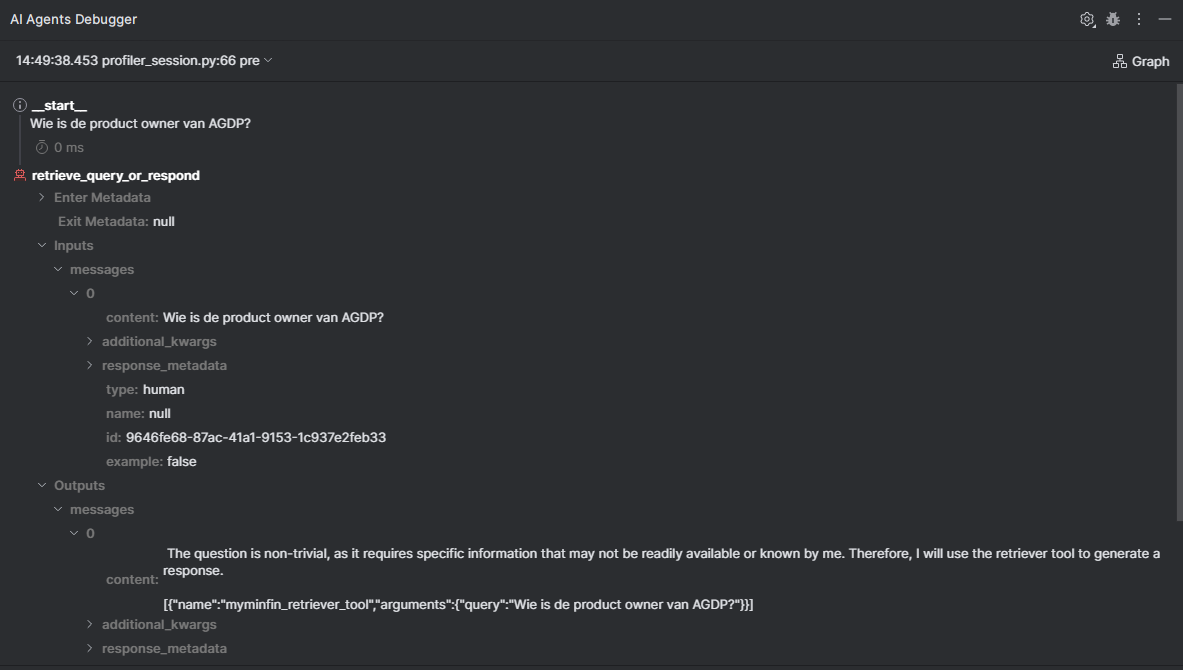
\includegraphics[width=0.8\textwidth]{mistral.png}
    \caption{Tool call bij het Mistral:7b model}
    \label{fig:Mistral}
\end{figure}

De figuur~\ref{fig:Mistral} illustreert waar het fout loopt bij dit model. Ondanks dat het model zich bewust is van de aanwezigheid van de tool en correct inschat dat de gestelde vraag niet triviaal is, wordt de tool-call toch niet effectief uitgevoerd.
\\[1em]
Opmerkelijk is dat de tool-call met de juiste parameters wel aanwezig is in de content van het antwoord, maar deze wordt niet als daadwerkelijke tool-call geïnterpreteerd of geactiveerd door het model.
\\[1em]
Dit probleem deed zich voor bij de volgende modellen:
\begin{itemize}
    \item Mistral-7b-instruct
    \item smollm2-1.7b-instruct
    \item granite-3.2-8b-instruct
    \item granite-3.3
\end{itemize}

 Daardoor kunnen deze modellen niet worden gebruikt binnen deze PoC en de bijhorende vergelijkende studie, aangezien ze de vectordatabase nooit aanspreken en dus geen relevante antwoorden aan de gebruiker kunnen bieden.

\subsection{Fout door oneindige herformuleringslus}

Hoewel de LLM in staat is om zelf te bepalen wat een non triviale vraag is, betekent dit niet noodzakelijk dat het antwoord daarop terug te vinden is in de beschikbare documentatie. Zelfs wanneer de informatie wel aanwezig is, kan het alsnog voorkomen dat de LLM, zelfs na herformulering van de vraag, geen passend antwoord weet te genereren. Dit leidde aanvankelijk tot een oneindige lus waarbij uiteindelijk een foutmelding werd gegenereerd zodra de array messages in de MessageState een lengte van 25 bereikte. In dat geval werd er geen antwoord aangemaakt, maar kreeg de gebruiker enkel een foutmelding te zien met stacktrace.
\\[1em]
Om te voorkomen dat het programma in een dergelijke oneindige lus terechtkomt, werd er een extra controle ingebouwd op het moment dat de LLM moet kiezen tussen het herformuleren van de vraag of het genereren van een antwoord. In de praktijk betekent deze controle dat de LLM de vraag maximaal twee keer mag herformuleren. Hierdoor wordt de vectordatabase in totaal maximaal drie keer bevraagd. Indien er na deze pogingen nog steeds geen relevante documenten worden teruggevonden, is het de bedoeling dat de LLM dit expliciet communiceert aan de gebruiker, zonder dat er sprake is van hallucinaties. 

\subsection{Meertaligheid documentatie}
%het gaat hier over het feit dat hij steeds de eerste vraag vertaalde naar het engels.
%Hoe heb je dat opgelost? Eventueel kort uitleggen als dat relevant is.
Bij het testen van de lus ontstond het probleem dat telkens enkel de originele vraag werd herschreven. Hierdoor werd bijvoorbeeld de oorspronkelijke vraag wel correct naar het Engels herschreven, maar bij iedere volgende iteratie werd opnieuw exact dezelfde vertaling gegenereerd. Er werd met vorige pogingen geen rekening gehouden.
\\[1em]
Om dit probleem op te lossen, werd de prompt in de \verb|rewrite_question| node aangepast zodat de LLM ook rekening kan houden met de eerder gestelde en herschreven vragen. Dit voorkomt herhaling en zorgt voor meer variatie in de gegenereerde vragen.
\\[1em]
Aangezien het grootste deel van de beschikbare documentatie in het Frans of Engels is geschreven, wordt de LLM eveneens aangemoedigd om de vraag eerst naar het Frans te herschrijven en vervolgens, indien nodig, naar het Engels.

\begin{lstlisting}[basicstyle=\small, frame=single, breaklines=true, postbreak=\mbox{\textcolor{red}{$\hookrightarrow$}\space}, escapeinside ={\%,}, escapechar={!}, numbers=left, language=Python, caption=Prompt om vraag te herschrijven]
REWRITE_QUESTION_PROMPT = (
    "You are assisting with improving a user's question related to Myminfin IT support.\n"
    "Conversation history so far (most recent last):"
    "\n ------- \n"
    "{questions}"
    "\n ------- \n"
    "Original question:"
    "\n ------- \n"
    "{original_question}"
    "\n ------- \n"
    "Rewrite the last question to make it short, clear, and easy to match with relevant documents in a vector database.\n"
    "- Keep the meaning and intent exactly the same.\n"
    "- Use simple, direct wording without adding unnecessary details.\n"
    "- If the question is in Dutch, rewrite and translate it to French.\n"
    "- If the question is in French, rewrite and translate it to English.\n"
    "- Avoid repeating previous questions word-for-word.\n"
    "- If it’s similar to a previous question, add only minimal context needed for distinction.\n"
    "- Return only the rewritten question."
)
\end{lstlisting}
\section{Samenvatting}

%Korte recap: wat is gebouwd en werkt zoals verwacht?
%Eventueel: wat is nog niet geïmplementeerd en waarom niet (scope, tijdsbeperkingen)?

Het eindresultaat van deze PoC is een chatinterface die kan worden gebruikt om gerichte vragen te stellen aan de IT-support voor MyMinfin. De toepassing werkt zoals verwacht: afhankelijk van de vraag worden relevante documenten opgehaald en wordt de nodige informatie aan de eindgebruiker verstrekt. Hoewel de hoeveelheid documentatie nog verder opgeschaald kan worden, vormt dit een sterke eerste stap in het opzetten van een ondersteunende tool voor de dagelijkse supportwerking.
\\[1em]
Toch zijn er ook enkele zaken die momenteel nog ontbreken. Zo zou het nuttig zijn indien de agent zelfstandig documentatie kan aanpassen of aanvullen. Dit zou ervoor zorgen dat de beschikbare informatie steeds up-to-date blijft, zonder dat hiervoor handmatige tussenkomst van gebruikers nodig is. Deze functionaliteit viel echter buiten de scope van deze PoC en kon, omwille van tijdsbeperkingen, niet worden gerealiseerd.
\\[1em]
Daarnaast beschikt de huidige LLM-toepassing niet over enige vorm van geheugen. Bij elke nieuwe vraag begint de LLM volledig van nul, zonder kennis van eerdere interacties binnen dezelfde sessie. Er is dus geen sprake van contextopbouw of het onthouden van vorige vragen en antwoorden, wat de gebruikservaring momenteel beperkt tot losstaande interacties.
%%=============================================================================
%% Resultaten
%%=============================================================================

\chapter{Resultaten}
\label{ch:resultaten}

%TODO In de caption van figuren altijd een conclusie, op te merken afwijking… opgeven


%ResponseRelevancy  Scores the relevancy of the answer according to the given question. Answers with incomplete, redundant or unnecessary information is penalized. Score can range from 0 to 1 with 1 being the best.

%Faithfulness The Faithfulness metric measures how factually consistent a response is with the retrieved context. It ranges from 0 to 1, with higher scores indicating better consistency.

% AnswerCorrectness  Measures answer correctness compared to ground truth as a combination of factuality and semantic similarity.

%LLMContextRecall checkt in hoeverre de juiste info voor het antwoord ook effectief aanwezig was in de opgehaalde context. Hoe meer overlap tussen juiste antwoord en context, hoe hoger de score.  aka hoe goed het model zijn retrievalproces heeft aangestuurd.

Om de verschillende modellen te testen, worden meerdere scenario’s gehanteerd.
Ten eerste wordt gebruikgemaakt van een testset met tien vragen waarvan de informatie beschikbaar is in de documentatie. Van elk model wordt verwacht dat het op iedere vraag een concreet antwoord geeft. Deze antwoorden worden vervolgens geëvalueerd met behulp van het test framework \textit{Ragas}, waarbij vier verschillende meetcriteria worden toegepast.
\\[1em]
Het tweede testscenario bestaat uit het stellen van niet-triviale vragen waarvoor de informatie niet beschikbaar is in de documentatie. Dit scenario is vooral bedoeld om te onderzoeken of bepaalde modellen tekenen van hallucinaties vertonen.
\\[1em]
Als laatste worden enkele triviale vragen gesteld. Hierbij wordt getest of het model in staat is een juiste inschatting te maken door direct te antwoorden, zonder onnodige zoekopdrachten in de vector database.

\section{Evaluatie 1: Documentatiegebaseerde vragen}

Voor elk model werd een afzonderlijke vragenlijst opgesteld, waarbij de verwachte antwoorden zijn opgenomen in bijlage \ref{vragenlijst}.
De antwoorden die door de modellen zijn gegenereerd, zijn weergegeven in bijlage \ref{antwoordenlijst}.
In beide bijlagen zijn, uit overwegingen van gegevensbescherming, alle contactgegevens geanonimiseerd.
\\[1em]
Voor deze evaluatie wordt gebruikgemaakt van een testframework Ragas. Tijdens de testen wordt voor iedere vraag de volgende informatie verzameld: de gebruikersinput, de opgehaalde context, het antwoord van de LLM en het verwachte antwoord. Op basis van deze gegevens gebruikt Ragas zelf een LLM om de dataset te beoordelen volgens de gekozen evaluatie criteria. In dit geval werd hiervoor het testmodel \textit{gemma3:4b} gebruikt, omdat dit model een goede balans biedt tussen rekensnelheid, geheugengebruik en beoordelingskwaliteit. Hierdoor kon de evaluatie efficiënt worden uitgevoerd. Dit resulteert in een rapport waarin iedere vraag wordt beoordeeld op de verschillende criteria.
\\[1em]
De scores per vraag variëren tussen 0 en 1, waarbij een score van 1 een volledig correct antwoord representeert.
Binnen de categorie \textit{Faithfulness} geeft een score van 0{,}000 aan dat het model ten onrechte heeft nagelaten de retriever-tool te gebruiken, waardoor de opgehaalde context leeg bleef.
Voor de categorie \textit{Context Recall} kan dit in sommige gevallen juist het tegenovergestelde effect hebben: wanneer de opgehaalde context leeg is, kan het antwoord van het model toch een score van 1 behalen, mits het volledig aansluit bij de afwezigheid van context.
\\[1em]
Het meetcriterium Faithfulness beoordeelt hoe consistent het antwoord is met de opgehaalde context. \textit{Response Relevancy} kijkt naar hoe relevant het antwoord is ten opzichte van de vraag. Onvolledige of overbodige informatie leidt hierbij tot een lagere score. \textit{Answer Correctness} beoordeelt hoe correct het antwoord is in vergelijking met het verwachte antwoord, waarbij zowel feitelijke als semantische overeenkomsten worden meegenomen. Context Recall controleert in welke mate de benodigde informatie voor het antwoord aanwezig is in de opgehaalde context. Hoe groter de overlap tussen het juiste antwoord en de context, hoe hoger de score. Dit meetcriterium kijkt dus vooral naar hoe goed het model het ophaalproces aanstuurt.
\\[1em]
Bij sommige modellen en vragen traden tijdens het testen errors op. Dit hield in dat de documentatie ofwel niet werd opgehaald, ofwel foutief uit de vectordatabase kwam. Voor deze vragen werd vastgesteld dat de meetcriteria Faithfulness en Response Relevancy een score van 0 kregen, terwijl bij voor Context Recall een 1 werd toegekend. Om een realistischer beeld van de prestaties van de modellen te geven, wordt voor deze vragen de Context Recall aangepast naar 0, aangezien dit beter weerspiegelt hoe het model daadwerkelijk presteerde voor die vraag. Deze correcties werden toegepast voor Llama3.1 vraag 4 en voor Qwen2.5 vragen 4, 7 en 9.
\\[1em]
%Vragen waar het model geen antwoord op kon bieden waren 1, 2, 7 en 10 Voor vragen 3, gaf het model wel een antwoord maar dit was niet in het geval van vraag 3 niet waarheidsgetrouw in het geval van vragen 5, lag het probleem eerder aan de documentatie die niet éénduidig was. Bij vraag 4 was er een error tijdens het RAG proces wat resulteerde in de slechte resultaten.
In tabel \ref{tab:resultaten_vragen_llama3.1} worden de resultaten van Llama3.1 weergegeven. Opvallend is dat de Response Relevancy in veel gevallen nul scoort, wat aangeeft dat de antwoorden van het model vaak niet relevant zijn voor de gestelde gebruikersvragen. Daarnaast blijft de score voor Answer Correctness over het algemeen laag. Dit valt deels te verklaren doordat het model voor een aantal vragen de nodige informatie niet kon vinden in de vectordatabase.
\\[1em]
Verder valt op dat het model, ondanks dat de juiste informatie in de context aanwezig is, vaak niet in staat is deze correct te combineren tot een juist antwoord. Een duidelijk voorbeeld hiervan is vraag 10. Hier was de Context Recall een 1, maar de Answer Correctness slechts 0.205. Het model gaf aan de vraag niet te kunnen beantwoorden, ondanks dat de benodigde informatie wel beschikbaar was in de context.

\begin{table}[H]
    \begin{tabular}{|l|c|c|c|c|}
        \hline
        \textbf{Vraag} & \textbf{Faithfulness} & \textbf{Response Relevancy} & \textbf{Answer Correctness} & \textbf{Context Recall} \\
        \hline
        Vraag 1 & 1.000 & 0.000 & 0.225 & 0.500 \\
        Vraag 2 & 0.333 & 0.000 & 0.221 & 0.000 \\
        Vraag 3 & 0.385 & 0.000 & 0.223 & 0.500 \\
        Vraag 4 & 0.000 & 0.000 & 0.174 & 0.000 \\
        Vraag 5 & 1.000 & 0.863 & 0.212 & 0.125 \\
        Vraag 6 & 0.667 & 0.920 & 0.477 & 1.000 \\
        Vraag 7 & 0.500 & 0.000 & 0.205 & 1.000 \\
        Vraag 8 & 0.714 & 0.000 & 0.408 & 1.000 \\
        Vraag 9 & 0.500 & 0.932 & 0.391 & 1.000 \\
        Vraag 10 & 0.333 & 0.000 & 0.205 & 1.000 \\
        \hline
    \end{tabular}
    \caption{Resultaten per vraag op de vier meetcriteria van het Llama3.1 model. De antwoorden blijken vaak niet relevant voor de vraag (Response Relevancy = 0), en de Answer Correctness blijft over het algemeen laag.}
    \label{tab:resultaten_vragen_llama3.1}
\end{table}

In tabel \ref{tab:resultaten_vragen_llama3.2} worden de resultaten van Llama3.2 weergegeven. Het meest opvallende resultaat is vraag 7, waar het model zeer hoge scores behaalt op alle criteria en bijna een perfecte score bereikt voor Answer Correctness (0.991). Daarnaast laat het model, ondanks de kleinere modelgrootte, toch degelijke prestaties zien.
\\[1em]
Ook de resultaten voor vraag 8 zijn opmerkelijk. Hier behaalt het model op bijna alle criteria een hoge score, met uitzondering van Answer Correctness. Dit verschil wordt veroorzaakt door de ambiguïteit in de opgehaalde documentatie. De bronnen boden geen eenduidig correct antwoord. Het door het model gegeven antwoord komt daardoor niet overeen met de ground truth, maar kan wel worden verantwoord op basis van de beschikbare documentatie.
\begin{table}[H]
    \centering
    \begin{tabular}{|l|c|c|c|c|}
        \hline
        \textbf{Vraag} & \textbf{Faithfulness} & \textbf{Response relevancy} & \textbf{Answer Correctness} & \textbf{Context Recall} \\
        \hline
        Vraag 1  & 0.500 & 0.894 & 0.485 & 0.500 \\
        Vraag 2  & 0.333 & 0.000 & 0.220 & 0.000 \\
        Vraag 3  & 0.800 & 0.000 & 0.219 & 0.500 \\
        Vraag 4  & 0.571 & 0.863 & 0.196 & 0.833 \\
        Vraag 5  & 0.625 & 0.000 & 0.205 & 0.125 \\
        Vraag 6  & 0.857 & 0.000 & 0.194 & 1.000 \\
        Vraag 7  & 0.917 & 0.860 & 0.991 & 1.000 \\
        Vraag 8  & 0.833 & 0.953 & 0.212 & 1.000 \\
        Vraag 9  & 0.429 & 0.883 & 0.631 & 0.375 \\
        Vraag 10 & 0.333 & 0.000 & 0.207 & 1.000 \\
        \hline
    \end{tabular}
    \caption{Resultaten per vraag op de vier meetcriteria van het Llama3.2 model. Opvallend is vraag 7, waar het model bijna perfecte scores behaalt op alle criteria. Bij vraag 8 werd vastgesteld dat ambiguïteit in de documentatie kan leiden tot een lage Answer Correctness, ondanks hoge scores op de andere criteria.}
    \label{tab:resultaten_vragen_llama3.2}
\end{table}

In tabel \ref{tab:resultaten_vragen_qwen2.5} worden de resultaten van Qwen2.5 weergegeven. Opvallend is dat de Response Relevancy vrijwel overal nul scoort en dat de Context Recall zeer laag is. De enige uitzondering is vraag 6, waar het model zowel de context correct ophaalt als een relevante respons genereert. Deze lage scores zijn deels het gevolg van errors tijdens het uitvoeren van het RAG-proces. Een andere reden is dat het model in sommige gevallen direct een antwoord formuleerde zonder eerst de vectordatabase te raadplegen. Ook blijft de score voor Answer Correctness voor de andere vragen relatief laag waardoor de prestaties van dit model niet overtuigend zijn.

\begin{table}[H]
    \begin{tabular}{|l|c|c|c|c|}
        \hline
        \textbf{Vraag} & \textbf{Faithfulness} & \textbf{Response relevancy} & \textbf{Answer Correctness} & \textbf{Context Recall} \\
        \hline
        Vraag 1  & 0.750 & 0.000 & 0.485 & 0.500 \\
        Vraag 2  & 0.500 & 0.000 & 0.226 & 0.000 \\
        Vraag 3  & 0.929 & 0.000 & 0.229 & 0.500 \\
        Vraag 4  & 0.000 & 0.000 & 0.174 & 0.000 \\
        Vraag 5  & 0.000 & 0.000 & 0.180 & 0.000 \\
        Vraag 6  & 1.000 & 0.871 & 0.469 & 1.000 \\
        Vraag 7  & 0.000 & 0.000 & 0.176 & 0.000 \\
        Vraag 8  & 0.000 & 0.000 & 0.179 & 0.000 \\
        Vraag 9  & 0.000 & 0.000 & 0.176 & 0.000 \\
        Vraag 10 & 0.667 & 0.000 & 0.216 & 0.000 \\
        \hline
    \end{tabular}
    \caption{Resultaten per vraag op de vier meetcriteria van het Qwen2.5 model. De Response Relevancy en Context Recall zijn vrijwel overal nul, met uitzondering van vraag 6 waar het model zowel de context correct ophaalt als een relevante respons geeft. Over alle vragen blijft de Answer Correctness laag, wat duidt op matige prestaties van dit model.}
    \label{tab:resultaten_vragen_qwen2.5}
\end{table}


In tabel \ref{tab:resultaten_vragen_qwen3} worden de resultaten van Qwen3 weergegeven. Voor dit model valt op hoe hoog de Faithfulness is wat betekent dat het model zich goed houdt aan de informatie die het heeft opgehaald en bijgevolg minder geneigd is om hallucinaties te vertonen. Het model scoort voor vraag 7 zeer hoog op alle categorieën. De Answer Correctness blijft bij enkele vragen echter laag. Voor vragen 1 tot en met 4 gaf het model aan geen antwoord te kunnen vinden in de context. Bij vraag 5 werd gedateerde informatie uit de vectordatabase opgehaald waardoor het antwoord niet overeenstemde met de ground truth. Voor vraag 9 werd slechts een deel van het correcte antwoord uit de database gehaald. Op basis van de opgehaalde context besloot het model een andere chunk te gebruikten om een antwoord te genereren. Dit resulteert in een lage Answer Correctness met op hetzelfde moment een hoge Faithfulness en een vrij hoge Context Recall.

\begin{table}[H]
    \begin{tabular}{|l|c|c|c|c|}
        \hline
        \textbf{Vraag} & \textbf{Faithfulness} & \textbf{Response Relevancy} & \textbf{Answer Correctness} & \textbf{Context Recall} \\
        \hline
        Vraag 1  & 1.000 & 0.000 & 0.216 & 0.500 \\
        Vraag 2  & 1.000 & 0.000 & 0.224 & 0.000 \\
        Vraag 3  & 1.000 & 0.000 & 0.220 & 0.250 \\
        Vraag 4  & 0.857 & 0.000 & 0.203 & 0.000 \\
        Vraag 5  & 0.636 & 0.867 & 0.211 & 0.125 \\
        Vraag 6  & 0.750 & 0.874 & 0.571 & 1.000 \\
        Vraag 7  & 1.000 & 0.906 & 0.989 & 1.000 \\
        Vraag 8  & 0.556 & 0.000 & 0.411 & 1.000 \\
        Vraag 9  & 1.000 & 0.000 & 0.340 & 0.625 \\
        Vraag 10 & 1.000 & 0.935 & 0.636 & 1.000 \\
        \hline
    \end{tabular}
    \caption{Resultaten per vraag voor het Qwen3 model waarbij opvalt dat Faithfulness hoog is en het model bij vraag 7 op alle meetcriteria hoge scores behaalt terwijl de Answer Correctness bij enkele vragen lager blijft door ontbrekende of gedateerde informatie.}
    \label{tab:resultaten_vragen_qwen3}
\end{table}


\subsection{Samenvatting}

Om de prestaties van de modellen per meetcriterium te vergelijken, worden in figuur~\ref{fig:vergelijking_metrics} vier staafdiagrammen weergegeven. Elk diagram toont de gemiddelde score van de verschillende modellen voor één specifiek meetcriterium.

\begin{figure}[H]
    \centering
    \begin{subfigure}{0.48\textwidth}
        \centering
        \begin{tikzpicture}
            \begin{axis}[
                ybar,
                ymin=0,
                ymax=1,
                bar width=8pt,
                width=\textwidth,
                height=0.6\textwidth,
                enlarge x limits=0.25,
                ylabel={Score},
                symbolic x coords={L3.1,L3.2,Q2.5,Q3},
                xtick=data,
                nodes near coords,
                nodes near coords align={vertical},
                every node near coord/.append style={font=\small},
                title={Faithfulness}
                ]
                \addplot coordinates {(L3.1,0.543) (L3.2,0.620) (Q2.5, 0.385) (Q3,0.880)};
            \end{axis}
        \end{tikzpicture}
    \end{subfigure}
    \hfill
    \begin{subfigure}{0.48\textwidth}
        \centering
        \begin{tikzpicture}
            \begin{axis}[
                ybar,
                ymin=0,
                ymax=1,
                bar width=8pt,
                width=\textwidth,
                height=0.6\textwidth,
                enlarge x limits=0.25,
                ylabel={Score},
                symbolic x coords={L3.1,L3.2,Q2.5,Q3},
                xtick=data,
                nodes near coords,
                nodes near coords align={vertical},
                every node near coord/.append style={font=\small},
                title={Response Relevancy}
                ]
                \addplot coordinates {(L3.1,0.272) (L3.2,0.445) (Q2.5,0.087) (Q3,0.358)};
            \end{axis}
        \end{tikzpicture}
    \end{subfigure}
    
    \vspace{1em}
    
    \begin{subfigure}{0.48\textwidth}
        \centering
        \begin{tikzpicture}
            \begin{axis}[
                ybar,
                ymin=0,
                ymax=1,
                bar width=8pt,
                width=\textwidth,
                height=0.6\textwidth,
                enlarge x limits=0.25,
                ylabel={Score},
                symbolic x coords={L3.1,L3.2,Q2.5,Q3},
                xtick=data,
                nodes near coords,
                nodes near coords align={vertical},
                every node near coord/.append style={font=\small},
                title={Answer Correctness}
                ]
                \addplot coordinates {(L3.1,0.274) (L3.2,0.356) (Q2.5,0.251) (Q3,0.402)};
            \end{axis}
        \end{tikzpicture}
    \end{subfigure}
    \hfill
    \begin{subfigure}{0.48\textwidth}
        \centering
        \begin{tikzpicture}
            \begin{axis}[
                ybar,
                ymin=0,
                ymax=1,
                bar width=8pt,
                width=\textwidth,
                height=0.6\textwidth,
                enlarge x limits=0.25,
                ylabel={Score},
                symbolic x coords={L3.1,L3.2,Q2.5,Q3},
                xtick=data,
                nodes near coords,
                nodes near coords align={vertical},
                every node near coord/.append style={font=\small},
                title={Context Recall}
                ]
                \addplot coordinates {(L3.1,0.613) (L3.2,0.633) (Q2.5,0.2) (Q3, 0.550)};
            \end{axis}
        \end{tikzpicture}
    \end{subfigure}
    
    \caption{Vergelijking van de gemiddelde scores per meetcriterium voor de modellen Llama3.1 (L3.1), Llama3.2 (L3.2), Qwen2.5 (Q2.5) en Qwen3 (Q3). De figuur toont dat Qwen3 de hoogste Faithfulness behaalt, terwijl de Response Relevancy en Answer Correctness bij de meeste modellen lager blijven. Context Recall varieert sterk tussen de modellen, waarbij Llama-modellen over het algemeen beter scoren dan Qwen2.5 en Qwen3.}
    \label{fig:vergelijking_metrics}
\end{figure}

Uit tabel \ref{tab:modelvergelijking} blijkt dat het model Qwen3 de hoogste scores behaalde voor Faithfulness (0.880) en Answer Correctness (0.402), terwijl Llama3.2 het beste presteerde op Response Relevancy (0.445) en Llama3.1 op Context Recall (0.713). 
\\[1em]
Opvallend is dat niet één model op alle gemeten criteria het beste scoorde. Zo behaalde het Qwen3 model de hoogste score op zowel Faithfulness als Answer Correctness. Dit suggereert dat dit model zich het meest consistent hield aan de geleverde context, en over de hele set van tien vragen ook de meest accurate antwoorden genereerde.
\\[1em]
Voor Response Relevancy was het Llama3.2 model de best presterende. De laagste score op dit meetcriterium werd echter behaald door het Qwen2.5 model, met een opvallend lage waarde van 0.087. Dit wijst erop dat de antwoorden van dit model vaak irrelevante of overbodige informatie bevatten, of dat cruciale elementen uit het antwoord ontbraken.
\\[1em]
Op het vlak van Context Recall scoorde het Llama3.2 model het hoogst, op korte afstand gevolgd door Llama3.1. Dit betekent dat Llama3.2 er het best in slaagde om relevante documentatie op te halen. Toch bleek dit niet automatisch te leiden tot een hoge Answer Correctness. Ondanks de hoge Context Recall, presteerde Llama3.2 niet het sterkste op vlak van Answer Correctness. In tegenstelling daarmee behaalde het Qwen3 model wel een hoge Answer correctness met een iets lagere Context Recall, wat impliceert dat het model de opgehaalde informatie beter wist te verwerken en toepassen.

\begin{table}[H]
    \begin{tabular}{|l|c|c|c|c|c|}
        \hline
        \textbf{Model} & \textbf{Faithfulness} & \textbf{Response Relevancy} & \textbf{Answer Correctness} & \textbf{Context Recall} \\
        \hline
        \textbf{Llama3.1} & 0.543 & 0.272 & 0.274 & 0.613 \\
        \textbf{Llama3.2} & 0.620 & \textbf{0.445} & 0.356 & \textbf{0.633} \\
        \textbf{Qwen2.5}  & 0.385 & 0.087 & 0.251 & 0.200 \\
        \textbf{Qwen3}    & \textbf{0.880} & 0.358 & \textbf{0.402} & 0.550 \\
        \hline
    \end{tabular}
    \caption{Vergelijking van modelprestaties op vier evaluatiecriteria. Qwen3 behaalt de hoogste gemiddelde scores, terwijl Llama3.2 de op één na hoogste score behaalt en bovendien relatief consistent presteert over de verschillende categorieën. Dit ondanks het kleinere aantal parameters.}
    \label{tab:modelvergelijking}
\end{table}

Figuur \ref{fig:gemiddelde_score_per_model_met_sd} geeft een overzicht van de gemiddelde score van elk model over de vier categorieën, waarbij elke categorie even zwaar meeweegt in de eindberekening. Op deze manier kunnen de verschillende modellen snel met elkaar worden vergeleken. Hoewel dit niet het hele verhaal verteld, sluit dit gemiddelde wel aan bij de individuele prestaties van de modellen.
\\[1em]
Gemiddeld scoorde Qwen3 het best, met Llama3.2 op de tweede plaats. Dit is opvallend aangezien Llama3.2 slechts drie miljard parameters heeft, tegenover de andere modellen die zeven à acht miljard parameters hebben.
\\[1em]
Figuur \ref{fig:gemiddelde_score_per_model_met_sd} illustreert tevens dat Llama3.2 de meest consistente prestaties vertoont over de vier categorieën. De foutbalken representeren de standaarddeviatie van de scores. Waarbij een kleinere waarde wijst op minder grote spreiding en daarmee op consistente prestaties over de verschillende meetcriteria. Het model combineert met andere woorden een relatief hoge gemiddelde score met een hoge mate van consistentie.

\begin{figure}[H]
    \centering
    \begin{tikzpicture}
        \begin{axis}[
            ybar,
            ymin=0,
            ymax=1,
            bar width=20pt,
            width=0.8\textwidth,
            height=0.5\textwidth,
            enlarge x limits=0.25,
            ylabel={Gemiddelde score},
            symbolic x coords={Llama3.1,Llama3.2,Qwen2.5,Qwen3},
            xtick=data,
            nodes near coords,
            nodes near coords align={vertical},
            every node near coord/.append style={font=\small}
            ]
            \addplot+[
            error bars/.cd,
            y dir=both,
            y explicit
            ] coordinates {
                (Llama3.1,0.426) +- (0,0.178)
                (Llama3.2,0.514) +- (0,0.136)
                (Qwen2.5,0.231) +- (0,0.124)
                (Qwen3,0.548)   +- (0,0.236)
            };
        \end{axis}
    \end{tikzpicture}
    \caption{Gemiddelde score per model over de vier categorieën, met foutbalken die de standaarddeviatie weergeven. Llama3.2 vertoont de meest consistente prestaties, terwijl Qwen3 het hoogste gemiddelde behaalt maar met grotere spreiding.}
    \label{fig:gemiddelde_score_per_model_met_sd}
\end{figure}

\section{Evaluatie 2: Hallucinaties}

Bij deze test krijgt ieder model een set van 5 vragen voorgeschoteld. Geen van deze vragen komt voor in de documentatie (zie bijlage \ref{hallucinatie-resultaten}) Dit heeft als doel om na te gaan welke modellen tekenen vertonen van hallucinaties en welke niet. 
\\[1em]
De vragenlijst is als volgt:

\begin{enumerate}
    \item Voor welke dienst is Jan Cabooter verantwoordelijk?
    \item Wat is de maximale bestandsgrootte (in MB) die via de repush voor RV kan worden verstuurd?
    \item Wat is de kost voor een Nationality change?
    \item Wat is de technical resource voor DQSS?
    \item Wat is het maximum aantal documenten die kunnen geraadpleegd worden bij myminfin
\end{enumerate}

\begin{table}[H]
    \begin{tabular}{|l|c|c|c|c|}
        \hline
        \textbf{Vraag} & \textbf{Llama3.1} & \textbf{Llama3.2} & \textbf{Qwen2.5} & \textbf{Qwen3} \\
        \hline
       Vraag 1 & Nee & Ja & Nee & Nee \\
       Vraag 2 & Nee & Ja & Ja & Ja \\
       Vraag 3 & Ja & Nee & Nee & Nee \\
       Vraag 4 & Nee & Ja & Nee & Nee \\
       Vraag 5 & Nee & Ja & Nee & Nee \\
        \hline
    \end{tabular}
    \caption{Resultaten hallucinatie test per model bij vragen die niet in de documentatie voorkomen (Ja = hallucinatie, Nee = geen hallucinatie). Uit de resultaten blijkt dat voornamelijk Llama3.2 frequent hallucinaties vertoont, terwijl de andere modellen dit nauwelijks doen.}
\end{table}

\noindent\textbf{Samenvatting:}  
\begin{table}[H]
    \begin{tabular}{|l|c|}
        \hline
        \textbf{Model} & \textbf{Hallucinatie (\%)} \\
        \hline
        Llama3.1 & 1/5 (20\%) \\
        Llama3.2 & 4/5 (80\%) \\
        Qwen2.5  & 1/5 (20\%) \\
        Qwen3    & 1/5 (20\%) \\
        \hline
    \end{tabular}
    \caption{Samenvatting hallucinatie test. Het percentage geeft aan hoe vaak een model hallucinaties vertoonde. Opvallend is dat Llama3.2 met 80\% veruit het vaakst hallucinaties genereerde, terwijl de andere modellen dit slechts in 20\% van de gevallen deden.}
\end{table}

Uit de resultaten blijkt dat Llama3.2 in 80\% van de gevallen hallucinaties vertoonde, terwijl de overige modellen dit slechts in 20\% van de gevallen deden.

\subsection{Bespreking van de resultaten}

De modellen Qwen3, Qwen2.5 en Llama3.1 vertoonden geen tekenen van hallucinaties. Ze hielden zich goed aan de instructie om geen extra informatie te verzinnen en zich uitsluitend te baseren op de gegevens die in de opgehaalde documenten stonden. Wel ondervond elk van deze modellen problemen bij het beantwoorden van één specifieke vraag. Na nader onderzoek bleek dat, wanneer het model de vraag in het Frans herschreef, de tool call niet altijd correct functioneerde. Het is niet meteen duidelijk waarom dit gebeurde, maar bij de andere vragen traden er bij deze modellen geen hallucinaties op.
\\[1em]
Het Llama3.2-model daarentegen maakte meerdere keren aannames en verzon informatie die niet in de documentatie stond. Dit is uiteraard onwenselijk en kan verstrekkende gevolgen hebben voor de medewerkers die de support verzorgen, wanneer zij deze informatie als juist beschouwen.

\subsubsection{Relevantie voor echte toepassingen}
%Hoe cruciaal is dit type vraag in de praktijk?

Aangezien de opgeleverde informatie wordt gebruikt voor het behandelen van specifieke IT-vragen van burgers over MyMinfin, is het van groot belang dat de modellen geen hallucinaties vertonen. Zelfs wanneer het model uitsluitend informatie levert aan de supportmedewerker, is het essentieel dat deze informatie waarheidsgetrouw is. Op zijn minst moet het model bij twijfel expliciet aangeven dat de benodigde informatie niet beschikbaar is. Op basis van deze test kan het Llama3.2-model niet realistisch worden ingezet.

\section{Evaluatie 3: Triviale vraagstelling}

Tijdens deze test kreeg ieder model een reeks van vijf triviale vragen voorgelegd. De resultaten werden bepaald door de stacktrace van ieder model te analyseren. Op die manier werd vastgesteld of het model de vraag direct beantwoordde of eerst onnodig RAG uitvoerde (zie bijlage \ref{triviale-vragen-resultaten}).
\\[1em]
De vragenlijst is als volgt:

\begin{enumerate}
    \item Hallo hoe gaat het?
    \item Hoeveel dagen zitten er in een week?
    \item Wat is 2 + 2?
    \item In welk land ligt Parijs?
    \item Hoeveel minuten zitten er in een uur?
\end{enumerate}

\begin{table}[H]
    \centering
    \begin{tabular}{|l|c|c|c|c|}
        \hline
        \textbf{Vraag} & \textbf{llama3.1} & \textbf{llama3.2} & \textbf{Qwen2.5} & \textbf{Qwen3} \\
        \hline
        Hallo hoe gaat het? & Nee & Nee & Ja & Ja \\
        Hoeveel dagen zitten er in een week? & Nee & Nee & Ja & Ja \\
        Wat is 2 + 2? & Nee & Nee & Ja & Ja \\
        In welk land ligt Parijs? & Nee & Nee & Ja & Ja \\
        Hoeveel minuten zitten er in een uur? & Nee & Nee & Ja & Ja \\
        \hline
    \end{tabular}
    \caption{Resultaten van het correcte gebruik van de graaf per model bij triviale vragen waarbij verwacht wordt dat een direct antwoord wordt gegeven zonder gebruik van RAG. Er is een duidelijk onderscheid tussen de Llama-modellen en Qwen-modellen. De Llama-modellen raadplegen bij iedere vraag de vectordatabase terwijl de Qwen-modellen dit achterwege laten zoals wordt verwacht bij triviale vragen.}
    
\end{table}

\noindent\textbf{Samenvatting:}  
\begin{table}[H]
    \begin{tabular}{|l|c|}
        \hline
        \textbf{Model} & \textbf{Correct (\%)} \\
        \hline
        Llama3.1 & 0/5 (0\%) \\
        Llama3.2 & 0/5 (0\%) \\
        Qwen2.5  & 5/5 (100\%) \\
        Qwen3    & 5/5 (100\%) \\
        \hline
    \end{tabular}
    \caption{Samenvatting van correct gebruik van de graaf per model. Qwen2.5 en Qwen3 volgden in alle gevallen het verwachte gedrag terwijl Llama3.1 en Llama3.2 dit niet deden.}
\end{table}

Uit de resultaten blijkt dat Qwen2.5 en Qwen3 alle triviale vragen direct beantwoordden, terwijl Llama3.1 en Llama3.2 in alle gevallen onnodige RAG uitvoerden.

\subsection{Bespreking van de resultaten}
%Verwachtte je een foutloos resultaat?
De resultaten waren in deze vrij duidelijk de twee Llama modellen slaagde er niet in om een onderscheid te maken tussen triviale en niet-triviale vragen. Dit leidde ertoe dat ze bij iedere vraag het hele ophaalproces gingen uitvoeren. De twee Qwen modellen daarentegen gingen wel meteen antwoorden op de triviale vragen. Met andere woorden is het contrast tussen de Qwen en Llama modellen tijdens deze test vrij groot.
\\[1em]
De resultaten waren in dit geval vrij duidelijk. De twee Llama-modellen slaagden er niet in onderscheid te maken tussen triviale en niet-triviale vragen. Dit leidde ertoe dat zij bij elke vraag het volledige ophaalproces uitvoerden. De twee Qwen-modellen daarentegen gaven direct antwoord op de triviale vragen. Met andere woorden: het contrast tussen de Qwen- en Llama-modellen was tijdens deze test aanzienlijk.
\\[1em]
Hoewel dit niet direct invloed heeft op de inhoudelijke correctheid van de antwoorden, heeft het wel gevolgen voor de performantie van de toepassing. Bij niet-triviale vragen duurt het beantwoorden aanzienlijk langer bij de Llama-modellen dan bij de Qwen-modellen, omdat bij de Llama-modellen telkens het ophaalproces wordt opgestart. Voor een consistente en snelle werking van de PoC zijn de Qwen-modellen daardoor beter geschikt dan de Llama-modellen.
%Kunnen deze fouten vermeden worden met betere prompting?


\section{Samenvatting}
%Doel: Alles samenbrengen en overkoepelend reflecteren.
In deze vergelijkende studie werden vier LLM-modellen getest op drie manieren. Met name het beantwoorden van vragen op basis van opgehaalde documentatie, het behandelen van vragen die niet in de documentatie voorkwamen en het omgaan met triviale vragen. Elk model werd bij iedere deeltest beoordeeld op zijn prestaties.
\\[1em]
Op basis van deze testen kan worden geconcludeerd dat Qwen3 het beste model is in deze vergelijkende studie. In de eerste test behaalde het model twee keer de hoogste score en één keer de op één na hoogste score. Daarnaast vertoonde het model geen hallucinaties en ging het op een correcte manier om met triviale vragen. Met andere woorden is dit het enige model dat in alle drie de testen aan de verwachtingen voldeed. Op basis van deze resultaten kan worden geconcludeerd dat Qwen3 binnen deze PoC de meest betrouwbare prestaties leverde.
\\[1em]
De PoC met het Qwen3-model dekt de meeste behoeften die in de requirement analyse naar boven kwamen. Ten eerste gaat het model goed om met meertaligheid. Er werden hieromtrent geen problemen vastgesteld, ondanks dat de opgehaalde documentatie soms in een andere taal was. Het model slaagde er consistent in om te antwoorden in de taal van de gebruiker. Daarnaast gaf het model aan wanneer het onvoldoende kennis had om een vraag te beantwoorden. Dit is van groot belang, aangezien het anders tot foutieve antwoorden kan leiden. Dit resultaat sluit aan bij de hoge score voor Faithfulness die Qwen3 behaalde. Wanneer het model een antwoord genereerde, vermeldde het bovendien vaak de bron van de informatie, wat positief is omdat de gebruiker de informatie op die manier kan verifiëren.  
\\[1em]
Een aantal van de behoeften zijn niet vervuld. Dit is voornamelijk het gevolg van beperkingen in de onderliggende graafstructuur of beschikbare documentatie en niet van het model zelf. Een concreet voorbeeld hiervan is de afwezigheid van een volwaardige chatfunctionaliteit binnen de PoC.
%%=============================================================================
%% Discussie
%%=============================================================================

\chapter{Discussie}
\label{ch:discussie}


%ResponseRelevancy  Scores the relevancy of the answer according to the given question. Answers with incomplete, redundant or unnecessary information is penalized. Score can range from 0 to 1 with 1 being the best.

%Faithfulness The Faithfulness metric measures how factually consistent a response is with the retrieved context. It ranges from 0 to 1, with higher scores indicating better consistency.

% AnswerCorrectness  Measures answer correctness compared to ground truth as a combination of factuality and semantic similarity.

%LLMContextRecall checkt in hoeverre de juiste info voor het antwoord ook effectief aanwezig was in de opgehaalde context. Hoe meer overlap tussen juiste antwoord en context, hoe hoger de score.  aka hoe goed het model zijn retrievalproces heeft aangestuurd.

\section{Documentatiegebaseerde vragen}

Binnen deze sectie worden de testresultaten besproken van de eerste evaluatie, namelijk de prestaties op vragen waarvan de antwoorden terug te vinden zijn in de documentatie.

\subsection{Interpretatie van de resultaten}

Opvallend is dat niet één model op alle gemeten criteria het beste scoorde. Zo behaalde het Qwen3 model de hoogste score op zowel \textit{Faithfulness} als \textit{Answer Correctness}. Dit suggereert dat dit model zich het meest consistent hield aan de geleverde context, en over de hele set van tien vragen ook de meest accurate antwoorden genereerde.
\\[1em]
Voor \textit{Response Relevancy} was het Llama3.2 model de best presterende. De laagste score op deze metric werd echter behaald door het Qwen2.5 model, met een opvallend lage waarde van 0.087. Dit wijst erop dat de antwoorden van dit model vaak irrelevante of overbodige informatie bevatten, of dat cruciale elementen uit het antwoord ontbraken.
\\[1em]
Op het vlak van \textit{Context Recall} scoorde het Llama3.1 model het hoogst, op korte afstand gevolgd door Llama3.2. Dit betekent dat Llama3.1 er het best in slaagde om relevante documentatie op te halen. Toch bleek dit niet automatisch te leiden tot een hoge \textit{Answer Correctness}. Ondanks de hoge context recall, presteerde Llama3.1 relatief zwak op het vlak van antwoordjuistheid. In tegenstelling daarmee behaalde het Qwen3 model wel een hoge answer correctness met een iets lagere context recall, wat impliceert dat het model de opgehaalde informatie beter wist te verwerken en toepassen.
\\[1em]
Over het algemeen scoorde het Qwen3 model het best, met het Llama3.2 model opvallend op de tweede plaats. Dat is opmerkelijk, aangezien Llama3.2 slechts beschikt over drie miljard parameters, terwijl de andere modellen zeven tot acht miljard parameters tellen. Op basis daarvan zou men verwachten dat Llama3.2 het zwakst zou presteren op de verschillende evaluatiemetrics, maar dat blijkt niet het geval.

\section{Vragen buiten documentatie}
Deze testen werden uitgevoerd om na te gaan of de modellen zouden gaan hallucineren. Door vragen te stellen die 

\subsection{Interpretatie van de resultaten}

Het Qwen3, Qwen2.5 en Llama3.1 model vertoonde geen tekenen van hallucinaties. Zij hielden zich goed aan de instructies om geen extra informatie aan te verzinnen en zich enkel te basseren op zaken die in de opgehaalde documenten stonden. Elk van deze modellen had wel voor elk een probleem bij het beantwoorden van de vraag. Na nader te bekijken wat hiervan aan de oorzaak lag kon worden vastgesteld dat wanneer het model de vraag ging herschrijven in het Frans de tool call niet altijd werkte zoals voorzien. Het is niet meteen duidelijk waarom dit gebeurde maar er was bij deze modellen voor de andere vragen geen andere gevallen van hallucinaties.

Het Llama3.2 model daarentegen ging verschillende keren assumpties maken en zaken gaan verzinnen die niet in de documentatie stonden. Dit is uiteraard niet de bedoeling en kan verstrekkende gevolgen hebben voor mensen die de support doen als ze deze zaken als waar beschouwen. 

\subsection{Relevantie voor echte toepassingen}
%Hoe cruciaal is dit type vraag in de praktijk?

%Wat zijn de risico’s als de tool een fout antwoord geeft?

\subsection{Beperkingen en bedenkingen}
%Kan het zijn dat de tool zich baseerde op training data?

%Hoe kan je dit in de toekomst verbeteren?

\section{Triviale vragen}
%Doel: Onderzoeken hoe het systeem omging met zeer eenvoudige of voor de hand liggende vragen.

\subsection{Verwachting versus resultaat}
%Verwachtte je een foutloos resultaat?

%Werden er toch fouten gemaakt?

\subsection{Implicaties van fouten (indien van toepassing)}
%Wat zegt dit over de betrouwbaarheid van het systeem?

%Kunnen deze fouten vermeden worden met betere prompting?

\section{Vergelijking en implicaties}
%Doel: Alles samenbrengen en overkoepelend reflecteren.

\subsection{Vergelijking tussen de drie categorieën}
%In welke categorie scoorde het systeem het best?

Welke categorie leverde de meeste problemen op?

\subsection{Algemene sterktes en zwaktes van het systeem}
%Wanneer werkt het goed? Wanneer niet?

%Is het geschikt voor professioneel gebruik?

\subsection{Implicaties voor praktijk/toekomstig onderzoek}
%Wat betekenen deze resultaten voor bedrijven of ontwikkelaars?

%Wat zou een logisch vervolgonderzoek zijn?

\section{Beperkingen van de studie}
%%=============================================================================
%% Aanbevelingen
%%=============================================================================

\chapter{Aanbevelingen}%
\label{ch:aanbevelingen}
%%=============================================================================
%% Conclusie
%%=============================================================================

\chapter{Conclusie}%
\label{ch:conclusie}

% Trek een duidelijke conclusie, in de vorm van een antwoord op de
% onderzoeksvra(a)g(en). Wat was jouw bijdrage aan het onderzoeksdomein en
% hoe biedt dit meerwaarde aan het vakgebied/doelgroep? 
% Reflecteer kritisch over het resultaat. In Engelse teksten wordt deze sectie
% ``Discussion'' genoemd. Had je deze uitkomst verwacht? Zijn er zaken die nog
% niet duidelijk zijn?
% Heeft het onderzoek geleid tot nieuwe vragen die uitnodigen tot verder 
%onderzoek?


% onderzoeksvra(a)g(en). Wat was jouw bijdrage aan het onderzoeksdomein en
% hoe biedt dit meerwaarde aan het vakgebied/doelgroep? 
% Reflecteer kritisch over het resultaat. In Engelse teksten wordt deze sectie
Dit onderzoek biedt een helder overzicht van de verschillende mogelijkheden om een virtuele assistent te ontwikkelen. De uitgevoerde literatuurstudie maakt het mogelijk om, afhankelijk van de specifieke usecase, een weloverwogen keuze te maken tussen de verschillende benaderingen. Daarnaast werd een PoC uitgewerkt die aantoont hoe één van deze benaderingen,in dit geval RAG, kan worden toegepast in de praktijk. Niet alleen de PoC, maar ook de problemen die zich stelde tijdens de ontwikkeling bieden waardevolle lessen voor iedereen die een vergelijkbare PoC wil realiseren.
\\[1em]
De resultaten tonen aan dat de keuze van het LLM-model een cruciale rol speelt. Niet elk model is geschikt voor elke taak, zoals duidelijk werd bij functionaliteiten zoals tool calling. Binnen deze studie konden echter enkel kleinere modellen worden getest, waardoor niet uitgesloten kan worden dat krachtigere varianten van dezelfde modellen deze beperkingen ook hebben.
\\[1em]
Heel wat aspecten binnen dit onderzoek werden proefondervindelijk getest. De keuzes die binnen deze PoC gemaakt werden, zijn echter niet per definitie de beste voor elke RAG usecase. Elke toepassing vraagt om een specifieke afweging, afhankelijk van context, noden en technische randvoorwaarden.
\\[1em]
Het zou daarom waardevol zijn om in vervolgonderzoek niet enkel modellen onderling te vergelijken, maar ook andere aspecten van een RAG-architectuur nader te analyseren. Een eerste voorbeeld is het effect van verschillende parsers op ongestructureerde bestanden. Het is interessant om na te gaan welke parser het best omgaat met complexe PDF-bestanden die niet uitsluitend uit tekst bestaan, zoals gescande documenten of formulieren met tabellen en grafieken.
\\[1em]
Een tweede mogelijk onderzoekspiste betreft de impact van verschillende retrieval-methodes. Momenteel zijn er vier methodes beschikbaar, elk met een eigen aanpak voor het ophalen van documenten uit de vectordatabase. Een vergelijking van deze methodes op vlak van nauwkeurigheid, snelheid en robuustheid kan waardevolle inzichten opleveren.
\\[1em]
Een derde mogelijkheid is het analyseren van het effect van modelgrootte. In dit onderzoek werden voornamelijk modellen gebruikt met een vergelijkbaar aantal parameters. Het zou echter interessant zijn om na te gaan hoe verschillende versies van eenzelfde model met meer of minder parameters presteren in een RAG-context. Dit kan duidelijkheid scheppen over de verhouding tussen prestaties en efficiëntie.
\\[1em]
Tot slot kan het ook waardevol zijn om alternatieven voor RAG te verkennen. Binnen dit onderzoek werd bewust gekozen voor een RAG aanpak, maar gezien de snelle evolutie van LLM's en de steeds grotere context die deze modellen ter beschikking hebben kan het relevant zijn om te onderzoeken hoe een CAG systeem functioneert en of dit een valabel alternatief kan vormen.
\\[1em]
Samenvattend toont deze bachelorproef aan dat RAG een haalbare en veelbelovende aanpak is voor de ontwikkeling van een LLM-gebaseerde IT-supportbot in de context van MyMinfin. De opgedane inzichten vormen een stevige basis voor verdere optimalisatie en uitbreiding van dergelijke toepassing in de toekomst.

%---------- Bijlagen -----------------------------------------------------------

\appendix

\chapter{Onderzoeksvoorstel}

Het onderwerp van deze bachelorproef is gebaseerd op een onderzoeksvoorstel dat vooraf werd beoordeeld door de promotor. Dat voorstel is opgenomen in deze bijlage.
 
\section*{Samenvatting}

 Binnen de IT-sector is het verlenen van support aan klanten een essentieel onderdeel van de dienstverlening. Dit proces kan echter veel tijd en middelen vergen, vooral binnen grote organisaties. Het is vaak een uitdaging om snel en adequaat antwoorden te bieden op vragen van klanten, wat resulteert in een aanzienlijke investering van resources. Tegelijkertijd verwachten klanten een snelle oplossing voor hun problemen. Het is daarom in het belang van zowel de organisatie als de klant om vragen efficiënt te beantwoorden.

Deze bachelorproef onderzoekt de mogelijkheden voor het ontwikkelen van een virtuele assistent die supportmedewerkers kan ondersteunen bij het vinden van relevante antwoorden. Door middel van interviews met betrokkenen wordt een analyse gemaakt van het huidige proces, met als doel de pijnpunten in het verwerken van supporttickets in kaart te brengen. Daarnaast worden via een grondige literatuurstudie de verschillende opties voor het inzetten van een virtuele supportassistent onderzocht. Het einddoel is het ontwikkelen van een proof of concept dat bijdraagt aan een efficiëntere verwerking van klantvragen en de ondersteuning van medewerkers bij het oplossen van deze problemen.

Het verwachte resultaat van dit onderzoek omvat enerzijds een overzicht van de mogelijkheden van een virtuele supportassistent, met aandacht voor wat praktisch haalbaar is en welke factoren daarbij een rol spelen. Anderzijds wordt op basis van een concrete casus een toepassing ontwikkeld in de vorm van een proof of concept (PoC). Er wordt verwacht dat dergelijke virtuele assistenten in veel gevallen een meerwaarde kunnen bieden, maar niet voor alle bedrijven. Afhankelijk van de specifieke behoeften en de manier waarop een organisatie een virtuele assistent wil inzetten, moet eerst grondig worden geanalyseerd of een dergelijke implementatie daadwerkelijk waarde toevoegt. Pas na een dergelijke analyse kan overwogen worden om een virtuele supportassistent te implementeren.

%---------- Inleiding ---------------------------------------------------------

% TODO: Is dit voorstel gebaseerd op een paper van Research Methods die je
% vorig jaar hebt ingediend? Heb je daarbij eventueel samengewerkt met een
% andere student?
% Zo ja, haal dan de tekst hieronder uit commentaar en pas aan.

%\paragraph{Opmerking}

% Dit voorstel is gebaseerd op het onderzoeksvoorstel dat werd geschreven in het
% kader van het vak Research Methods dat ik (vorig/dit) academiejaar heb
% uitgewerkt (met medesturent VOORNAAM NAAM als mede-auteur).
% 

\section{Inleiding}%
\label{sec:inleiding}

Een ontwikkelingsteam heeft diverse verantwoordelijkheden. Naast hun primaire taak, het ontwikkelen van software, is het ook essentieel dat ze documentatie aanleveren. Dit kan variëren van API-documentatie voor andere teams tot een beginnersgids voor nieuwe medewerkers. Het is belangrijk dat deze documentatie steeds up-to-date blijft. Dit vormt echter niet de enige uitdaging; de documentatie moet ook overzichtelijk zijn en zo gestructureerd dat gebruikers eenvoudig de benodigde informatie kunnen vinden. Naarmate de tijd verstrijkt, wordt dit vaak steeds moeilijker te realiseren.

De beoogde doelgroep voor dit onderzoek bestaat uit IT-teams of organisaties die werken met een grote hoeveelheid documentatie, waarbij het soms een uitdaging is om snel specifieke informatie terug te vinden. Een virtuele assistent zou hier kunnen helpen door direct antwoorden te geven of gebruikers te verwijzen naar de relevante documentatie. Dit kan leiden tot duidelijkere inzichten in gedocumenteerde afspraken en daarmee een efficiëntere werking van het IT-team.

Het doel van dit onderzoek is om de mogelijkheden voor de ontwikkeling van een virtuele document-assistent te verkennen. Het onderzoek start met een literatuurstudie om verschillende opties en mogelijke beperkingen in kaart te brengen. Vervolgens wordt een Proof of Concept (POC) ontwikkeld, die als eerste stap dient richting de implementatie van een document-assistent.

%---------- Stand van zaken ---------------------------------------------------

\section{Stand van zaken}%
\label{sec:stand van zaken}

Hier beschrijf je de \emph{state-of-the-art} rondom je gekozen onderzoeksdomein, d.w.z.\ een inleidende, doorlopende tekst over het onderzoeksdomein van je bachelorproef. Je steunt daarbij heel sterk op de professionele \emph{vakliteratuur}, en niet zozeer op populariserende teksten voor een breed publiek. Wat is de huidige stand van zaken in dit domein, en wat zijn nog eventuele open vragen (die misschien de aanleiding waren tot je onderzoeksvraag!)?

Je mag de titel van deze sectie ook aanpassen (literatuurstudie, stand van zaken, enz.). Zijn er al gelijkaardige onderzoeken gevoerd? Wat concluderen ze? Wat is het verschil met jouw onderzoek?

Verwijs bij elke introductie van een term of bewering over het domein naar de vakliteratuur, bijvoorbeeld~\autocite{Hykes2015}! Denk zeker goed na welke werken je refereert en waarom.

Draag zorg voor correcte literatuurverwijzingen! Een bronvermelding hoort thuis \emph{binnen} de zin waar je je op die bron baseert, dus niet er buiten! Maak meteen een verwijzing als je gebruik maakt van een bron. Doe dit dus \emph{niet} aan het einde van een lange paragraaf. Baseer nooit teveel aansluitende tekst op eenzelfde bron.

Als je informatie over bronnen verzamelt in JabRef, zorg er dan voor dat alle nodige info aanwezig is om de bron terug te vinden (zoals uitvoerig besproken in de lessen Research Methods).

% Voor literatuurverwijzingen zijn er twee belangrijke commando's:
% \autocite{KEY} => (Auteur, jaartal) Gebruik dit als de naam van de auteur
%   geen onderdeel is van de zin.
% \textcite{KEY} => Auteur (jaartal)  Gebruik dit als de auteursnaam wel een
%   functie heeft in de zin (bv. ``Uit onderzoek door Doll & Hill (1954) bleek
%   ...'')

Je mag deze sectie nog verder onderverdelen in subsecties als dit de structuur van de tekst kan verduidelijken.

%---------- Methodologie ------------------------------------------------------
\section{Methodologie}%
\label{sec:methodologie}


Voor het opstarten van deze bachelorproef is een literatuurstudie essentieel om bestaande mogelijkheden op het gebied van virtuele assistenten te verkennen. De literatuurstudie richt zich op een vergelijkende analyse die inzicht moet bieden in de verschillende beschikbare opties voor het opzetten van een eigen virtuele assistent. Hierbij is het belangrijk om de voor- en nadelen van elke optie in kaart te brengen, zodat op basis van deze informatie een weloverwogen keuze kan worden gemaakt voor de uitwerking van een proof of concept. Deze studie zal tevens duidelijkheid moeten verschaffen over de benodigde hardware- en softwarevereisten voor het ontwikkelen van de proof of concept.

Voor de realisatie van de proof of concept is een frontend nodig, waarvoor een IDE zoals Visual Studio Code essentieel is om de frontend-ontwikkeling te ondersteunen. Daarnaast is een GitHub-repository nodig voor versiebeheer en samenwerking.

Voor mijn bachelorproef zijn zowel de vergelijkende studie als de proof of concept essentieel. Daarom zullen beide onderdelen elk de helft van de beschikbare tijd in beslag nemen, wat betekent dat de vergelijkende studie een periode van twee maanden krijgt, en ook voor de ontwikkeling van de proof of concept twee maanden zijn voorzien. Hoewel het mogelijk is dat tijdens de eerste twee maanden al ideeën worden verkend voor de proof of concept, of dat er tijdens de ontwikkeling van de proof of concept nog aanpassingen aan de vergelijkende studie plaatsvinden, is het wel de bedoeling om eerst een gedegen vergelijkende studie op te stellen. Deze vergelijkende studie dient als basis voor de verdere uitwerking van de proof of concept.

%---------- Verwachte resultaten ----------------------------------------------
\section{Verwacht resultaat, conclusie}%
\label{sec:verwachte_resultaten}

Het verwachte resultaat van deze bachelorproef is tweeledig. Enerzijds wordt er een vergelijkende studie opgesteld, die voor bedrijven kan dienen als leidraad bij de implementatie van virtuele documentatie-assistenten en hen inzicht biedt in de verschillende mogelijkheden. Het is daarbij essentieel dat de vergelijkende studie niet alleen de technische aspecten behandelt, maar ook de financiële en juridische factoren in kaart brengt.

Anderzijds zal een proof of concept worden ontwikkeld als illustratie van een van de mogelijke opties binnen dit domein. Hiermee wordt de vergelijkende studie praktisch toegepast en vormt het een voorbeeld voor personen of organisaties die een soortgelijk project willen realiseren.

Bedrijven die te maken hebben met uitdagingen op het gebied van knowledge management kunnen deze vergelijkende studie benutten om te bepalen welke oplossing het beste bij hun behoeften past. Bovendien biedt de proof of concept, indien relevant en toepasbaar, de mogelijkheid om als basis te dienen voor een eigen implementatie, waarbij aanpassingen kunnen worden gemaakt om deze optimaal af te stemmen op de specifieke bedrijfscontext. Indien de proof of concept voldoende functioneel blijkt, kan deze een meerwaarde vormen door bestaande kennis en documentatie op een efficiënte en intuïtieve manier toegankelijk te maken voor medewerkers.

Het uiteindelijke onderzoeksresultaat zal een op ChatGPT lijkende interface opleveren, waarmee gebruikers gerichte antwoorden kunnen krijgen op vragen die specifiek betrekking hebben op hun organisatie. Deze oplossing richt zich dus op een bedrijfsspecifieke virtuele assistent, die getraind is op basis van de interne documentatie van een organisatie en binnen die context wordt ingezet.





%%---------- Andere bijlagen --------------------------------------------------
% TODO: Voeg hier eventuele andere bijlagen toe. Bv. als je deze BP voor de
% tweede keer indient, een overzicht van de verbeteringen t.o.v. het origineel.
\chapter{Bijlagen}
\section{Vragenlijst en verwacht antwoord}
\label{vragenlijst}

\begin{enumerate}
    \item \textbf{Wie is de product owner van AGDP en kan je de contactgegevens geven?} \\
    De product owner van AGDP is XXXXXXX en je kan haar contacteren via \texttt{XXXXXXX@XXXXXXX.be}.
    
    \item \textbf{Wie is de product owner van AGPR en kan je de contactgegevens geven?} \\
    De product owner van AGPR is XXXXXXX
    en je kan hem contacteren via \texttt{XXXXXXX@XXXXXXX.be}.
    
    \item \textbf{Kan je me alle contactgegevens geven voor het fragment UBO-register, ook de SNOW groep?} \\
    Fragment: UBO-register – Contactgegevens
    \begin{itemize}
        \item ICT:
        \item Group SNOW: TRES\_GRP\_CIFI
        \item Service manager: XXXXXXX (back-up: XXXXXXX)
        \item Business:
        \item Business analyst: XXXXXXX
    \end{itemize}
    
    \item \textbf{Hoe of waar moet ik mijn tijd loggen voor de support?} \\
    Where to log support time (from most preferred to least preferred):
    \begin{enumerate}
        \item Related ticket
        \begin{itemize}
            \item Project: MYMINFIN
            \item Log time to an existing issue whenever possible.
        \end{itemize}
        \item New bug
        \begin{itemize}
            \item Project: MYMINFIN
            \item If the reported problem requires creating a bug issue, log your time in an “analysis” subtask.
        \end{itemize}
        \item Business Support
        \begin{itemize}
            \item Fisc: [MYMINFIN-9958] [support] MYMINFIN 3rd line AGFISC/AAFISC - JIRA Cloud – ACTIVE
            \item Rec: MYMINFIN-12102: Recouvrement Support – ACTIVE
            \item Patdoc: MYMINFIN-12104: PatDoc Support – ACTIVE
            \item Douane: MYMINFIN-12106: Douane Support – ACTIVE
            \item Trésorerie: MYMINFIN-12108: Trésorerie Support – ACTIVE
            \item (Until end of August, except FISC)
        \end{itemize}
        \item Transversal Support (last resort if none of the above applies)
        \begin{itemize}
            \item Transversal: MYMINFIN-12182: Transversal Support – ACTIVE
            \item ICT: MYMINFIN-12110: Support Day – ACTIVE
            \item (Until end of August)
        \end{itemize}
    \end{enumerate}
    
    \item \textbf{Een gebruiker heeft geen toegang tot een functionaliteit wat moet ik hiermee doen?} \\
    Vragen met betrekking tot toegangsrechten moeten voortaan worden doorgestuurd naar de algemene mailboxen van de IAM-cellen.\\
    \textbf{Let op:} deze adressen MOGEN NIET aan klanten worden meegedeeld.\\
    Fiscaliteit: XXXXXXX@XXXXXXX.be\\
    Invordering \& Innen: XXXXXXX@XXXXXXX.be \\
    Patrimoniumdocumentatie: XXXXXXX@XXXXXXX.be\\
    Douane \& Accijnzen: XXXXXXX@XXXXXXX.be\\
    Thesaurie: XXXXXXX@XXXXXXX.be\\
    Algemeen: XXXXXXX@XXXXXXX.be
    
    \item \textbf{Er is een probleem met attest service, wie kan ik hiervoor contacteren?} \\
    Je kan contact opnemen met het development team via \texttt{XXXXXXX@XXXXXXX.be}.
    
    \item \textbf{Hoe doe ik een repush voor RV?} \\
    Hier zijn de stappen die gevolgd moeten worden wanneer het RV-team vraagt om een “repush” uit te voeren:
    \begin{enumerate}
        \item Open MyMinfin Civil Servant in een incognitovenster.
        \item Open een tweede tabblad en zet er alvast: \texttt{http://www.finbel.intra/}
        \item Zorg ervoor dat u over de volgende informatie beschikt:
        \begin{itemize}
            \item Application Type
            \item Status
            \item ID
        \end{itemize}
        \item In het tweede tabblad, plak een link met de volgende structuur achter:\\
          \begin{verbatim}
              {http://www.finbel.intra/myminfin-rest/myminfin-files-stirint
                  /put-in-queue/\{applicationType\}/\{status\}/\{id\}}
          \end{verbatim}
        Voorbeeld:\begin{verbatim}{myminfin-rest/myminfin-files-stirint/put-in-queue-by-id
                /WITHHOLDING\_TAX/VALIDATED/204832}\end{verbatim}
        \textbf{Opmerking:} Als u het volledige adres van de aanvrager krijgt, let er dan op dat er niet te veel spaties in staan.
        \item Druk op ENTER.
        \item Als alles goed verlopen is, geeft het systeem een succesbericht terug dat gecombineerd moet zijn met de melding 'queued files: 1'.\\
        Voorbeeld: 
        \begin{verbatim}
            {"restMessages":[{"type":"SUCCESS",
                    "bundleKey":"queued files : 1",...}]}
        \end{verbatim}
      \end{enumerate}
        
        \item \textbf{Iemand wil een document verwijderen dat hij heeft opgeladen via MyMinfin, wat kan ik hierop antwoorden?} \\
        Je kan het volgende antwoorden: MYMINFIN slaat geen gegevens op. Als het proces niet toelaat om te annuleren, moet de gebruiker contact opnemen met de afdeling die het document heeft ontvangen.\\
        Ik vermoed dat dit document is verstuurd via Antwoord op een brief - in dit geval moet de klant de gebruikte driecijferige code meedelen en moet je het ticket doorsturen naar het SOH-team. Die kunnen je vertellen met welke bevoegde service contact moet worden opgenomen.\\
        Wij kunnen u niet helpen.
        
        \item \textbf{Een burger kan werkt bij een onderneming, maar kan niet inloggen in de naam van de onderneming, wat moet ik hierop antwoorden?} \\
        Indien u niet de wettelijke vertegenwoordiger van de onderneming bent, hebt u een rol nodig om in te loggen in MYMINFIN in naam van uw eigen onderneming (inclusief filialen).\\
        U wilt in MYMINFIN toegang tot:
        \begin{itemize}
            \item de berichten van de onderneming, dan hebt u de rol FODFIN Berichten van de onderneming nodig;
            \item de documenten en formaliteiten van de onderneming, dan hebt u meestal genoeg aan de rol FOD Fin Aanstelling Eigen Onderneming met één of meerdere parameters in functie van uw verantwoordelijkheden (bv. Om de BTW formaliteiten te beheren, hebt u de parameter ‘Aanstelling BTW' nodig).
            \end{itemize}
Indien uw onderneming meerdere filialen telt, hebt u enkel de rol nodig die volstaat voor elk van die ondernemingen. Vergeet het begrip ‘mandaten'. Die zijn niet nodig als het om uw eigen onderneming (inclusief filialen) gaat.\\
Voor meer informatie kan u de volgende websites raadplegen:
\begin{itemize}
\item Welke rol ik moet toekennen : Rollen
\item Hoe toekennen of aanvragen van een rol : Beheer van de toegangsaanvragen in de rollenadministratie- RMA - Loginhulp.be
\end{itemize}
Eens dit in orde is, logt u aan op MyMinfin en identificeert zich “in naam van een onderneming”.\\
Selecteer uw eigen onderneming (of een filiaal).

\item \textbf{Wat zijn de contactgegevens voor de hypoimage service?} \\
service : AGDP - HYPOIMAGE \\
contacts : \texttt{XXXXXXX@XXXXXXX.be} ou PATDOC-RZSJ-Hypo (1e lijn) \\
- XXXXXXX@XXXXXXX.be (ICT - servicemanager ad interim) \\
- XXXXXXX@XXXXXXX.be (ICT - développeur)
\end{enumerate}


%%---------- Backmatter, referentielijst ---------------------------------------

\backmatter{}

\setlength\bibitemsep{2pt} %% Add Some space between the bibliograpy entries
\printbibliography[heading=bibintoc]

\end{document}
